% TODO: 
% - Zusammenfassung
% - lambda stetig in t_2, warum?
% - Interne Randpunkte, max halbe seite
% - Motivation Riccati gegenüber voherigen Beispielen: Beliebige quadratische Kostenfunktionale führen zu unlösbaren DGL --> riccati
% Anmerkung, dass Methode häufig auch gesamtheitlich als Maximumprinzip bezeichnet wird.

\chapter{Trajektorienoptimierung mit indirekten Methoden\index{Indirekte Optimierung}} \label{chap:dynamische_Optimierung_indirekt}
% Lösungen für stark einfache Probleme, potential sehr schneller lösungen (z.B. als Heuristik)
% Gute Vorlage: föllinger: grenzen der klassischen Lösungsmethode
Bei der Parameteroptimierung (s.\ Abschn.\,\ref{sec:statischeOptimierung}) ist bei einfachen Problemstellungen häufig die Anwendung der Differentialrechnung zielführend. So wird bereits Oberstufenschülern gelehrt, dass an den Extrema einer (differenzierbaren) Funktion $f(x)$ die erste Ableitung verschwindet, d.h. $f'(x) = 0$. % oder allgemein 
Im multivariaten Fall $\nabla\!f(\bs x) = \bs 0$ wird hierdurch ein Gleichungssystem erhalten, dessen Lösung \emph{indirekt} zu den Minima oder Maxima von $f(\bs x)$ führt. Analog hierzu wird bei der Variationsrechnung auf die Maxima oder Minima eines Funktionals $J(\bs x(t))$ geschlossen, indem kleine Änderungen $\delta J$ von der angenommenen Lösung betrachtet werden. Die Anwendung auf Optimalsteuerungsprobleme führt über die sog.\ \emph{Hamilton-Differentialgleichungen}\index{Hamilton-Gleichungen} auf ein \emph{Randwertproblem}\index{Randwertproblem}. Dessen Formulierung und Lösung hinsichtlich der Fahrzeuganwendung ist Kernstück des vorliegenden Kapitels.

Zum besseren Verständnis der Methodik werden zunächst für ein allgemeines, unbeschränktes Optimalsteuerungsproblem die für die Lösung notwendigen Gleichungen hergeleitet, was klassisch durch die Konstruktion von einparametrigen Vergleichskurvenscharen geschieht. Dadurch wird das Variationsproblem\index{Variationsrechnung} auf ein statisches Optimierungsproblem zurückgeführt, dessen allgemeine Lösung auf die Hamilton-Differentialgleichungen führt. \\
Anschließend werden die aus der Literatur bekannten Gleichungen für eine erweiterte Problemstellung mit End-, Punkt-, Eingangs- und Zustandsbeschränkungen vorgestellt und anhand von Beispielen aus dem Bereich der Trajektorienoptimierung von Fahrzeugen erläutert. Eine zentrale Stellung nimmt hierbei das sog.\ \emph{Maximumprinzip\index{Maximumprinzip} von Pontryagin} ein \cite{foellingeroptimal, papageorgiou2012optimierung}. \\
Schließlich wird das allgemeine Vorgehen bei der Klasse der \emph{linear-quadratischen} Optimierungsprobleme erläutert, für welche effiziente Lösungen existieren. Auf deren Basis wird ein neuer Algorithmus für das automatische Ausweichen vorgestellt, der eine Trajektorienoptimierung im Millisekundenbereich ermöglicht. Der entsprechende Abschnitt~\ref{seq:lqr_beispiel} wurde bereits in großen Teilen in der eigenen Arbeit \citeltex{werling2014riccati} veröffentlicht und übernommene Texte sind nicht gesondert gekennzeichnet.

%Die entsprechenden Kapitelinhalte wurden bereits im Rahmen von \citeltex{werling2014riccati} veröffentlicht.

Insgesamt erweist sich die im vorliegenden Kapitel vorgestellte Methodik zwar als vergleichsweise aufwändig in der Anwendung hinsichtlich der Berücksichtigung von Nebenbedingungen, bei einer geeigneten Problemformulierung ermöglicht sie jedoch eine äußerst effiziente Berechnung der Optimallösung auf heutigen Seriensteuergeräten. 


\section{Unbeschränkte Optimierungsprobleme}
% Vereinfachte Aufgabenstellung, Anwendung Fahrzeug: Berücksichtigung der NB in Kosten, oder Einbettung in übergeordnete Algorithmus

\subsection{Problemlösung mittels Variationsrechnung\index{Variationsrechnung}}\label{sec:herleitung_hamiltongleichungen}
Zur Verdeutlichung der Herangehensweise seien die Endzeit $t_f$ und der Endzustand $\bs{x}_f$ fest vorgegeben, aber keine weiteren Beschränkungen dem System auferlegt. Damit haben die Endkosten $V(\bs{x}(t_f))$ keinen Einfluss auf die Lösung, und das Optimalsteuerungsproblem \eqref{equ:optimalsteuerungsproblem} von S.\,\pageref{equ:optimalsteuerungsproblem} stellt sich folgendermaßen dar:
\begin{subequations} \label{equ:optimalsteuerungsproblem_}
\begin{align}
	\underset{\bs{u}(\cdot)}{\text{minimiere}}  \quad & %J(\bs{\phi}(t,\bar{\bs{u}}),\bs{\psi}(t,\bar{\bs{u}}),t)) = 
	\int_{t_0}^{t_f} l(\bs{x}(t),\bs{u}(t),t)\,{\rm d} t \\
		\label{equ:indir_sys}
	\text{u.B.v.} \quad & \dot{\bs x} = \bs f(\bs x, \bs u, t)\\
	& \bs x(t_0) = \bs x_0 \label{euq:anfangsbedingung}\\
	& \bs x(t_f) = \bs{x}_f \label{euq:endbedingung}
\end{align} 
\end{subequations}
Zur Berücksichtigung der Nebenbedingung $\bs f(\bs x, \bs u, t)  - \dot{\bs x} = \bs 0$ wird nun auf die sog.\ \emph{Lagrange-Multiplikatoren}\index{Lagrange-Multiplikator} zurückgegriffen, mit deren Hilfe ein Extremwertproblem mit Nebenbedingungen auf ein solches ohne Nebenbedingungen zurückgeführt werden kann \cite{foellingeroptimal, papageorgiou2012optimierung, graichen2014SkriptOpt}. Das Kostenfunktional stellt sich damit als
\begin{align} \label{equ:kosten_lagrange}
	\tilde J = \int_{t_0}^{t_f} \left[ l(\bs{x}(t),\bs{u}(t),t) + \bs \lambda ^\T(t) \, [\bs f(\bs x, \bs u, t) - \dot{\bs x} ] \right]{\rm d} t %+ V(\bs{x}(t_f))
\end{align}
dar. Im Unterschied zum Einsatz von konstanten Lagrange-Multiplikatoren in der statischen Optimierung ist der Vektor $\bs \lambda (t) = [ \lambda_1(t), \lambda_2(t), \ldots, \lambda_n(t) ]^\T$ bei der dynamischen Optimierung eine Funktion der Zeit. Er wird als \emph{Kozustand} oder \emph{adjungierte Variable} bezeichnet. \\
Es sei angenommen, dass die Lösung für $\bs x^\ast(t)$ und $\bs u^\ast(t)$ bekannt ist, womit einparametrische Vergleichskurvenscharen 
\begin{align*}
\bs x(t) &= \bs x^\ast(t) + \varepsilon\, \delta \bs x(t) \\
\bs u(t) &= \bs u^\ast(t) + \varepsilon\, \delta \bs u(t)
\end{align*}
auf $t \in [t_0, t_f]$  konstruiert werden, mit denen sich das Variationsproblem im Folgenden auf ein statisches Optimierungsproblem reduzieren lässt\footnote{Das Herangehen erscheint zunächst sehr ähnlich zur endlichen Parametrierung der direkten Optimierungsmethode aus Kap.\,\ref{chap:dynamische_Optimierung_direkt}, verfolgt aber einen ganz anderen Zweck, der erst später ersichtlich wird.}. Hierbei sind für $\delta \bs x(t)$ und $\delta \bs u(t)$ beliebige Zeitfunktionen zulässig,  die zu Vergleichskurven führen, die den Randbedingungen genügen, d.h.\ $\delta\bs x(t_0) = \bs 0$ und $\delta\bs x(t_f) = \bs 0$, s.\ Abb.\,\ref{fig:vergleichskurven}. Einsetzen dieser sog.\ \emph{zulässigen Variationen} in \eqref{equ:kosten_lagrange} liefert
\begin{figure}[t]
	\psfrag{1}[tc][tc][1.0]{$t_0$}
	\psfrag{2}[tc][tc][1.0]{$t_f$}
	\psfrag{t}[tc][tc][1.0]{$t$}
	\psfrag{3}[bc][bc][1.0]{$\bs x(t_0) = \bs x_0$}
	\psfrag{4}[bc][bc][1.0]{$\bs x(t_f) = \bs x_f$}
	\psfrag{e}[cr][cr][1.0]{$\varepsilon$}
	\psfrag{v}[bl][bl][1.0]{$\bs x^\ast(t) + \varepsilon\,\delta \bs x(t)$}
	\psfrag{o}[tl][tl][1.0]{$\bs x^\ast(t)$}
	\psfrag{x}[tl][tl][1.0]{$x$}
	\centering
  	\includegraphics[width=0.98\textwidth,clip, trim = 0cm 0cm 0cm 0cm]{6_variation_herleitung.eps}
	\caption[Zulässige Variationen um die optimale Lösung]{Zulässige Variationen um die optimale Lösung $\bs x^\ast(t)$ halten die Anfangs- und Endbedingungen ein, vgl. \cite{foellingeroptimal}.}
	\label{fig:vergleichskurven}
\end{figure} 
%
\begin{align} \label{equ:kosten_variation}
	\!\!\!\!\!\!\!\!\!\!\!\! \tilde J(\varepsilon)  \! =  \!\!\!\int_{t_0}^{t_f} \!\left[ l(\bs x^\ast \!\!+\! \varepsilon \delta \bs x,\bs u^\ast \!\!+\! \varepsilon \delta \bs u,t) + \bs \lambda ^\T [\bs f(\bs x^\ast \!\!+\! \varepsilon \delta \bs x, \bs u^\ast \!\!+\! \varepsilon \delta \bs u, t) - [\dot{\bs x}^\ast \!\!+\! \varepsilon \delta \dot{\bs x}] ] \right]\!{\rm d} t
	%+ V(\bs x^\ast(t_f) \!\!+\! \varepsilon \delta \bs x(t_f))
\end{align}
Da $\bs x^\ast(t)$ und $\bs u^\ast(t)$ die Lösung darstellt, muss $\tilde J(\varepsilon)$ für $\varepsilon = 0$ ein Minimum besitzen. Das wiederum bedeutet, dass es \emph{notwendig} ist, dass die erste Variation von $\tilde J$ Null ist, d.h.\ 
$\delta \tilde J := \left. \frac{{\rm d} \tilde J}{{\rm d} \varepsilon} \right|_{\varepsilon = 0} = 0$. Differentiation von \eqref{equ:kosten_variation} nach $\varepsilon$ und Einsetzen von $\varepsilon=0$ liefert (ohne Sternindex)
\begin{align*}
	\delta \tilde J  =  \!\!\! \int_{t_0}^{t_f} \bigg[  \bigg[ \frac{\partial l}{\partial \bs x} + \bigg[ \frac{\partial \bs f}{\partial \bs x}\bigg]^\T \!\!\! \bs \lambda\bigg]^\T \!\!\! \delta \bs x + \bigg[ \frac{\partial l}{\partial \bs u} + \bigg[ \frac{\partial \bs f}{\partial \bs u}\bigg]^\T \!\!\! \bs \lambda\bigg]^\T \!\!\! \delta \bs u - \bs \lambda^\T \delta \dot {\bs x}\bigg]{\rm d} t \; ,
\end{align*}
was durch Produktintegration\footnote{auch als partielle Integration bekannt: $\int_a^b v'(t) w(t) {\rm d} t = [v(t) w(t)]|_a^b - \int_a^b v(t) w'(t) {\rm d} t$ } zu
\begin{align*}
	\delta \tilde J  =  \!\!\! \int_{t_0}^{t_f} \left[  \bigg[ \frac{\partial l}{\partial \bs x} + \bigg[ \frac{\partial \bs f}{\partial \bs x}\right]^\T \!\!\! \bs \lambda + \dot {\bs \lambda} \bigg]^\T \!\!\! \delta \bs x + \bigg[ \frac{\partial l}{\partial \bs u} + \bigg[ \frac{ \partial \bs f}{\partial \bs u}\bigg]^\T \!\!\! \bs \lambda\bigg]^\T  \!\!\! \delta \bs u\bigg] {\rm d} t - \left.\left[\bs \lambda^T \delta \bs x\right]\right|_{t_0}^{t_f}
\end{align*}
führt. Aufgrund der Anfangs- und Endbedingungen gilt
\begin{align}
	\left.\left[\bs \lambda^T \delta \bs x\right]\right|_{t_0}^{t_f} = \bs \lambda(t_f)^\T \delta \bs x(t_f) - \bs \lambda ( t_0)^\T \delta \bs x(t_0) = 0 \;,
\end{align}
sodass  der letzte Term verschwindet. Da $\delta \tilde J = 0$ für alle zulässigen $\delta \bs x(t)$ und $\delta \bs u(t)$ gelten muss, sind folgende Gleichungen zu erfüllen:
\begin{subequations} \label{equ:herl_opt}
\begin{align}
\dot {\bs \lambda} 	&= -\frac{\partial l}{\partial \bs x} - \left[\frac{\partial f}{\partial \bs x}\right]^\T \bs \lambda\\
\bs 0     					&= \frac{\partial l}{\partial \bs u} + \left[\frac{\partial f}{\partial \bs u}\right]^\T \bs \lambda
\end{align}
\end{subequations}
Mit anderen Worten muss es zur optimalen Lösung  $\bs x^\ast(t)$ und $\bs u^\ast(t)$ auf $t_0 \leq t \leq t_f$ ein $\bs \lambda^\ast(t)$ geben, sodass die Gleichungen \eqref{equ:herl_opt} erfüllt sind.

\subsection{Hamilton-Gleichungen\index{Hamilton-Gleichungen} und Transversalitätsbedingungen\index{Transversalitätsbedingung}}
Die Systemdynamik \eqref{equ:indir_sys} und die im vorherigen Abschnitt hergeleiteten Gleichungen \eqref{equ:herl_opt} lassen sich mit Hilfe der sog.\ Hamilton-Funktion \cite{foellingeroptimal}
\begin{align}
H(\bs x, \bs u, \bs \lambda, t) = l(\bs x, \bs u, t) + \bs \lambda ^\T \bs f(\bs x, \bs u, t) \label{equ:hamitonfunktion}
\end{align}
auf dem Intervall $t_0 \leq t \leq t_f$ kompakt darstellen als
\begin{subequations} \label{equ:hamiltongl}
\begin{alignat}{3}
\dot {\bs x} 				&= \bs f(\bs x, \bs u, t) & &\Rightarrow & \dot {\bs x} &= \,\,\,\, \frac{\partial H}{\partial \bs \lambda}  \label{equ:hamilton_dgl}\\
\dot {\bs \lambda} 	&= -\frac{\partial l}{\partial \bs x} - \left[\frac{\partial \bs f}{\partial \bs x}\right]^\T \bs \lambda \quad & &\Rightarrow \quad  & \dot {\bs \lambda} &=  -\frac{\partial H}{\partial \bs x} \label{equ:hamilton_dgl_adj}\\
\bs 0     					   &= \,\,\,\,  \frac{\partial l}{\partial \bs u} + \left[\frac{\partial \bs f}{\partial \bs u}\right]^\T \bs \lambda & &\Rightarrow & \bs 0 &=  \,\,\,\, \frac{\partial H}{\partial \bs u}  \; . \label{equ:hamilton_steuergleichung}
\end{alignat}
\end{subequations}
Die Gleichungen \eqref{equ:hamiltongl} stellen entsprechend der Herleitung \emph{notwendige} Bedingungen an eine optimale Lösung dar und werden auch als \emph{Hamilton-Gleichungen}\index{Hamilton-Gleichungen} oder \emph{kanonische Gleichungen} bezeichnet. \\
Aufgrund der festen Anfangs- und Endvorgabe im Optimalsteuerungsproblem \eqref{equ:optimalsteuerungsproblem_} muss zusätzlich die Lösung noch 
\begin{align}
\bs x(t_0) = \bs x_0 \label{equ:fester_anfangszustand}\\
\bs x(t_f) = \bs x_f \label{equ:fester_endpunkt}
\end{align}
genügen.

In vielen Fahrsituationen können jedoch der Endzustand und der Endzeitpunkt eines Manövers im Vorfeld der Optimierung gar nicht so genau spezifiziert werden, sodass sie Teil der Optimierung werden. Der Endzustand unterliegt dann dennoch bestimmten Bedingungen, da z.B. das Fahrzeug am Ende des Manövers entlang der Straße ausgerichtet sein muss, s.\ später Abschn.\,\ref{sec:polytraj}. Zu diesem Zweck können, anstelle von \eqref{equ:fester_endpunkt}, sog.\ \emph{Zielmannigfaltigkeiten}\index{Zielmannigfaltigkeit}
\begin{align}
	\bs g(\bs x(t_f), t_f) = \bs 0 \label{equ:zm_indiropt}
\end{align}
vorgegeben werden, die bereits im Optimalsteuerungsproblem \eqref{equ:optimalsteuerungsproblem} auf S.\,\pageref{equ:optimalsteuerungsproblem} in \eqref{equ:zm} aufgeführt sind. 
Damit haben aber die Endkosten $V(\bs{x}(t_f))$ im Kostenfunktional \eqref{equ:opt_funktional} wieder Einfluss auf die Lösung, sodass es häufig zielführend ist, über sie "`Empfehlungen"' bzgl.\ des Endzustands zu formulieren.
Die zulässigen Variationen $\delta \bs x(t)$ müssen jetzt \eqref{equ:zm_indiropt} genügen, sodass analog zu Abschn.\,\ref{sec:herleitung_hamiltongleichungen} mit neuem Lagrange-Multiplikator\index{Lagrange-Multiplikator} $\bs \mu = \text{const.}$ die Bedingung
\begin{align} \label{equ:trans_x}
\left[\frac{\partial V}{\partial \bs x}\right]_{t_f} - \bs \lambda(t_f) + \left[\frac{\partial \bs g}{\partial \bs x}\right]_{t_f}^\T \bs \mu = \bs 0
\end{align}
hergeleitet werden kann. Falls keine Vorgaben bzgl.\ des Endzustands gemacht werden sollen, es wird auch von freiem Endzustand gesprochen, dann gilt
\begin{align} \label{equ:trans_x_frei}
\bs \lambda(t_f) = \left[\frac{\partial V}{\partial \bs x}\right]_{t_f} \;.
\end{align}


%oder falls ganz frei
%\begin{align*}
%\left[\frac{\partial V}{\partial \bs x}\right]_{t_f} - \bs \lambda(t_f) = \bs 0
%\end{align*}
Ist die Endzeit $t_f$ frei, so ergibt sich durch Variation um die optimale Endzeit $t_f^\ast$  der Zusammenhang
%\begin{subequations} 
\begin{align} \label{equ:trans_t}
%\left[\frac{\partial V}{\partial t}\right]_{t_f} &+ \left[H(\bs x, \bs u, \bs \lambda, t)\right]_{t_f}  = 0 \quad \text{falls $\bs x(t_f)$ fest, ansonsten} \\
\left[\frac{\partial V}{\partial t}\right]_{t_f} &+ \left[H(\bs x, \bs u, \bs \lambda, t)\right]_{t_f} + \left[\frac{\partial \bs g}{\partial \bs t}\right]_{t_f}^\T \bs \mu = 0\; ,
\end{align}
der sich für einen freien Endzustand zu
\begin{align}
	\left[\frac{\partial V}{\partial t}\right]_{t_f} &+ \left[H(\bs x, \bs u, \bs \lambda, t)\right]_{t_f}  = 0 \label{equ:trans_t_freies_x}
\end{align}
%\end{subequations}
vereinfacht.
Gleichungen \eqref{equ:trans_x} und \eqref{equ:trans_t} stellen sog. \emph{Transversalitätsbedingungen}\index{Transversalitätsbedingung} dar \cite{papageorgiou2012optimierung, foellingeroptimal, graichen2014SkriptOpt}.

Des Weiteren sind interne Randpunkte\index{interner Randpunkt} \cite{papageorgiou2012optimierung} von Interesse, da Not-Manöver typischerweise so zu planen sind, dass das Fahrzeug eine Kollision zu einem bestimmten Zeitpunkt $t_1$ vermeidet, bevor es das Manöverende bei $t_f$ erreicht, s.\ hierzu später Abb.\,\ref{fig:Lokale_Koordinate_Ausweichen}. Da können analog zu den Endkosten $V(\bs x(t_f),t_f)$ in \eqref{equ:opt_funktional} zusätzlich Punktkosten für einen internen Randpunkt in $t_1$ veranschlagt werden, sodass sich insgesamt
\begin{align*}
	\tilde J(\bs x(t), \bs u(t), t_f, t_1) = J(\bs x(t), \bs u(t), t_f) + \tilde V(\bs x(t_1),t_1)
\end{align*}
ergibt. Des Weiteren kann es ebenfalls zweckmäßig sein, Gleichungsnebenbedingungen der Form 
\begin{align*}
	\tilde {\bs g}(\bs x(t_1),t_1) = \bs 0
\end{align*}
zu berücksichtigen. Durch Variation um den optimalen internen Zustand $\bs x_1^\ast$ und den optimalen Zeitpunkt $t_1^\ast$ ergeben sich \cite{papageorgiou2012optimierung} die zusätzlichen Transversalitätsbedingungen
\begin{align}
\bs \lambda(t_1^-) &= \bs \lambda(t_1^+) + \left[\frac{\partial \tilde  V}{\partial\bs x}\right]_{t_1} + \left[\frac{\partial \tilde {\bs g}}{\partial\bs x}\right]_{t_1}^\T  \bs\nu \label{equ:interne_randpunkte_lambda} \\
\left[H(\bs x, \bs u, \bs \lambda, t)\right]_{t_1^-} &= \left[H(\bs x, \bs u, \bs \lambda, t)\right]_{t_1^+} - \left[\frac{\partial \tilde  V}{\partial t}\right]_{t_1} - \left[\frac{\partial \tilde {\bs g}}{\partial t}\right]_{t_1}^\T  \bs\nu \;, \label{equ:interne_randpunkte_H}
\end{align}
wobei $t_1^-$ und $t_1^+$ die Zeit unmittelbar vor und nach $t_1$ bezeichnen. Entfallen die Gleichungsnebenbedingungen, so ist in den Gleichungen $\bs \nu=\bs 0$ zu setzen. Es erklärt sich von selbst, dass $\bs x(t)$ in $t_1$ stetig verlaufen muss.

Zusammenfassend kann festgehalten werden, dass, wenn es eine optimale Lösung $\bs x^\ast(t)$ und $\bs u^\ast(t)$ gibt, dann muss sie den Hamilton-Gleichungen \eqref{equ:hamiltongl}, den festen Anfangsbedingungen \eqref{equ:fester_anfangszustand} und Endbedingungen \eqref{equ:fester_endpunkt}  bzw.\ Transversalitätsbedingungen \eqref{equ:trans_x},\eqref{equ:trans_t} und ggf.\ \eqref{equ:interne_randpunkte_lambda} und \eqref{equ:interne_randpunkte_H}  genügen. Umgekehrt reicht es nicht in jedem Fall, das Randwertproblem der Hamilton-Gleichungen zu lösen, um zur Optimalsteuerungslösung zu gelangen. Sie stellen entsprechend der Herleitung nur notwendige Bedingungen dar. Aus Entwicklersicht muss die Aufgabenstellung daher so formuliert werden, dass es nur eine Lösung geben kann. Ist das nicht möglich, so kann häufig das Kostenfunktional jeder Lösung des Randwertproblems evaluiert werden, um so zur optimalen Lösung zu gelangen.

\subsection{Anwendung auf optimalen Spurwechsel} \label{sec:polytraj}
% Föllinger, Graichen
% Hamilton-Gleichungen nur notwendig. Es können zwar 2. Variation betrachtet werden, in der Praxis reicht aber scharfes Nachdenken meist aus.
% Numerische Verfahren möglich, aber bei einfachen Problemen auch geschlossene Lösungen möglich -> s. restliches Kapitel
% Direkte Schießverfahren, etc.
Zur Lösung eines Optimalsteuerungsproblems wird generell mit der Steuergleichung \eqref{equ:hamilton_steuergleichung} begonnen, die als gewöhnliche  $m$-dimensionale Gleichung $\bs x, \bs \lambda, \bs u$ und $t$ in Beziehung setzt und daher auch als \emph{Koppelgleichung} bezeichnet wird. Um den Systemeingang in den Hamilton-Gleichungen zu eliminieren, muss sie nach $\bs u$ aufgelöst werden %, 
%\begin{align}
	%\bs u = \bs \psi(\bs x, \bs \lambda, t) \; , \label{equ:solve_u}
%\end{align}
%was i.Allg.\ möglich ist\footnote{todo}. 
% papageorgiou2012optimierung Seite 193
und anschließend in die $n$-dimensionale Zustandsgleichung des Systems \eqref{equ:hamilton_dgl}
 und in die $n$ Differentialgleichungen für den Kozustand $\bs \lambda$ eingesetzt werden. Insgesamt entstehen $2n$ verkoppelte, von $\bs u$ unabhängige Differentialgleichungen 1.\ Ordnung. \\
In Kombination mit den $2n$ Randbedingungen, die neben dem Anfangszustand \eqref{equ:fester_anfangszustand} entweder durch eine Endvorgabe \eqref{equ:fester_endpunkt} oder durch die Transversalitätsbedingung \eqref{equ:trans_x} gegeben sind, und zusätzlich \eqref{equ:trans_t}, sofern  $t_f$ frei ist, entsteht ein \emph{Randwertproblem}\index{Randwertproblem}, das durch verschiedene Methoden \cite{papageorgiou2012optimierung, Graichen2012} numerisch gelöst werden kann. Der große Vorteil der Indirekten Optimierungsmethode besteht jedoch darin, dass für einfache aber elementare Aufgabenstellungen das Randwertproblem analytisch gelöst werden kann und damit zu einem sehr schnell ausführbaren Algorithmus führt.

Die Herangehensweise sei anhand eines optimalen Spurwechsels verdeutlicht, vgl.\ \citeltex{werling2012optimal} und \cite{Hult2013Thesis}. Vereinfachend wird nur die Querbewegung des Fahrzeugs relativ zur Zielfahrspur betrachtet, sodass der Fahrzeugzustand der Differentialgleichung eines dreifachen Integrators mit $\bs x = [x_1, x_2, x_3]^\T$ und
\begin{align*}
	\dot{\bs x} = \bs f(\bs x, u) = [x_2, x_3, u ]^\T
\end{align*}
genügt, wobei der Ruck als Eingang $u$ dient und der Koordinatenursprung in der Mitte der Zielspur liegt, s.\ Abb.\,\ref{fig:polytraj}. \\

\begin{figure}[h]
\centering
	\psfrag{t}[bc][bc]{$s(t)$}
	\psfrag{1}[cr][cr]{$x_1$}
	\psfrag{x}[cc][cc]{$\bs x^\ast$}
	\psfrag{0}[ct][ct]{$\bs x_0$}
	\psfrag{a}[cb][cb]{\scriptsize (a)}
	\psfrag{b}[ct][ct]{\scriptsize (b)}
	\psfrag{c}[ct][ct]{\scriptsize (c)}
	\psfrag{e}[bc][bc]{$t_f^\ast$}
	\centering
  	\includegraphics[width=.8\textwidth,clip, trim = 0cm 0cm 0cm 0cm]{6_Polytraj.eps}
  \caption[Ruck-optimaler Spurwechsel]{Ruck-optimaler Spurwechsel mit (a) festem Endzustand und (b) freiem Endzustand; Ruck-Zeit-optimaler Spurwechsel (c) mit freiem Endzustand und freier Endzeit $t_f$; Zur Veranschaulichung sind die Trajektorien in Abhängigkeit der zurückgelegten Wegstrecke $s(t)$ für $v=\text{const.}$ dargestellt \citeltex{werling_handbook}.}
    \label{fig:polytraj}
\end{figure}

\textbf{Fester Endzustand} \\
Gesucht wird zunächst die optimale Zustandstrajektorie $\bs x^\ast(t)$ auf dem Intervall $0\leq t \leq t_f$, sodass der gegebene Anfangszustand 
\begin{align}
	\bs x(0) = \bs x_0 \label{equ:x_0}
\end{align} bis zum festen Zeitpunkt $t_f$ in den Endzustand
\begin{align}
\bs x(t_f) = \bs 0 \;, \label{equ:x_f}
\end{align}
also auf der neuen Fahrbahnmitte ohne verbleibende Querbewegung, übergeführt wird, s.\ Trajektorie (a) in Abb.\,\ref{fig:polytraj}. Hierbei soll das komfortmotivierte Gütefunktional 
%(s.\ auch Abschn.\,\ref{sec:...})
\begin{align}
	J &= %\int_{0}^{t_f}l(u(t)) {\rm d} t = 
	\int_{0}^{t_f}\frac{1}{2} u(t)^2 {\rm d} t \label{equ:integrator_J}
\end{align}
minimiert werden, wobei o.B.d.A.\ $t_0$ zu Null gesetzt wurde. 
Mit der Hamilton-Funktion \eqref{equ:hamitonfunktion}
\begin{align*}
	H = %l + \bs \lambda^\T \bs f = 
	\frac{1}{2}u^2 + \lambda_1 x_2 + \lambda_2 x_3 + \lambda_3 u
\end{align*}
ergibt sich die Steuergleichung \eqref{equ:hamilton_steuergleichung} zu
\begin{align}
	0 &=  \frac{\partial H}{\partial u} = u + \lambda_3 \quad \Rightarrow \quad u = -\lambda_3 \;. \label{equ:integrator_u}
\end{align}
Die Kozustandsdifferentialgleichung \eqref{equ:hamilton_dgl_adj} wiederum liefert
\begin{align*}
	\dot {\bs \lambda} =  -\frac{\partial H}{\partial \bs x} = %\mtrx{ccc}{0 & 0 & 0 \\ 1 & 0 & 0 \\ 0 & 1 & 0} \cdot \mtrx{c}{\lambda_1 \\ \lambda_2 \\ \lambda_3} =  
	\mtrx{c}{0 \\ \lambda_1 \\ \lambda_2}
\end{align*}
und damit gilt
\begin{alignat}{3}
\nonumber
	\dot \lambda_1 &= 0 \quad  & &\Rightarrow &\quad \lambda_1(t) &= c_1 \\
\nonumber
	\dot \lambda_2 &= \lambda_1 & &\Rightarrow  & \lambda_2(t) &= c_1 t + c_2 \\
\label{equ:lambda_3}
	\dot \lambda_3 &= \lambda_2 & &\Rightarrow  & \lambda_3(t) &= \frac{1}{2}c_1 t^2 + c_2 t + c_3 \; , 
\end{alignat}
was mit dem Integrationskonstanten-Vektor $\bs c_1 = [c_1, c_2, c_3]^\T $ kompakt in Matrixschreibweise als
\begin{align*}
	 \bs \lambda(t) = \bs M_1(t) \bs c_1	\quad \text{mit} \quad \bs M_1(t) = \mtrx{ccc}{1 & 0 & 0 \\ t & 1 & 0 \\ \tfrac{1}{2} t^2 & t & 1}
\end{align*}
dargestellt werden kann.
%
Des Weiteren ist $u$ mittels \eqref{equ:integrator_u} in \eqref{equ:hamilton_dgl} zu eliminieren, sodass
\begin{align*}
	\dot {\bs x} = \mtrx{c}{x_2 \\ x_3 \\ -\lambda_3} \,,
\end{align*}
woraus
\begin{alignat*}{3}
	\dot x_3 &= -\lambda_3 \;\;  & &\Rightarrow &\;\; x_3(t) &= -\frac{1}{6}c_1 t^3 - \frac{1}{2}c_2 t^2 - c_3 t - c_4 \\
	\dot x_2 &= x_3 & &\Rightarrow  & x_2(t) &= -\frac{1}{24} c_1 t^4 - \frac{1}{6}c_2 t^3 - \frac{1}{2} c_3 t^2 - c_4 t - c_5 \\
	\dot x_1 &= x_2 & &\Rightarrow  & x_1(t) &= -\frac{1}{120} c_1 t^5 - \frac{1}{24} c_2 t^4 - \frac{1}{6}c_3 t^3 -\frac{1}{2}c_4 t^2 - c_5 t - c_6
\end{alignat*}
folgt, was sich als
\begin{align*}
	 &\bs x(t) = \bs M_2(t) \bs c_1 + \bs M_3(t) \bs c_2 \quad \text{mit} \quad 
	 \bs M_2(t) = \mtrx{ccc}{-\frac{1}{120} t^5 & -\frac{1}{24} t^4 & -\frac{1}{6} t^3 \\ 
	                         -\frac{1}{24}  t^4 & -\frac{1}{6}  t^3 & -\frac{1}{2} t^2 \\ 
													 -\frac{1}{6}   t^3 & -\frac{1}{2}  t^2 & -            t  }, \\
													%
 &\bs M_3(t) = - \bs M_p\cdot \bs M_1(t), \quad \bs M_p = \mtrx{rrr}{ 0 & 0 & 1 \\ 0 & 1 & 0 \\ 1 & 0 & 0} \quad \text{und} \quad \bs c_2 = [c_4, c_5, c_6]^\T
\end{align*}
repräsentieren lässt. Unter Berücksichtigung der Anfangsbedingungen \eqref{equ:x_0} ergibt sich mit $\bs M_2(0) = \bs 0$ und $\bs M_3(0) = -\bs M_p$ direkt $\bs c_2 = -\bs M_p \bs x_0$, sodass
\begin{align}
	 &\bs x(t) = \bs M_2(t) \bs c_1 - \bs M_3(t) \bs M_p \bs x_0 \; . \label{equ:x_of_t}
\end{align}
Damit stellt sich die Endvorgabe \eqref{equ:x_f} als
\begin{align}
	\bs x(t_f)  = \bs M_2(t_f) \bs c_1 - \bs M_3(t_f) \bs M_p \bs x_0 = \bs 0 \label{equ:x_of_t_f}
\end{align}
dar, was durch Auflösen nach den verbleibenden Integrationskonstanten 
\begin{align*}
  \bs c_1 = \bs M_2(t_f)^{-1} \bs M_3(t_f) \bs M_p \bs x_0\; , \quad  t_f \neq 0
\end{align*}
liefert, sodass die optimale Trajektorie $\bs x^\ast(t)$ bestimmt ist. \\

\textbf{Freier Endzustand} \\
Aufgrund von $\bs M_2(0) = \bs 0$ entsteht im vorhergehenden Optimierungsproblem für $t_f=0$ eine Singularität, die sich in der Anwendung darin äußert, dass im optimierungsbasierten Regelkreis gegen Ende des Manövers das Fahrzeug auf kleinste Störungen und Messrauschen zunehmend nervös reagiert, da es um jeden Preis (Stellgröße) die Endvorgabe erreichen muss. Da das Fahrzeug gar nicht angewiesen ist, exakt in der Fahrspurmitte zu fahren, kann das Problem durch Optimierung über den Endzustand gelöst werden.
%Hierzu sei nun nicht mehr der Endzustand vollständig vorgegeben, sondern nur noch
%\begin{align*} \label{equ:integrator_g}
	%\bs g(\bs x(t_f), t_f) = [x_2(t_f), x_3(t_f)]^\T = \bs 0 \;,
%\end{align*}
%sodass der Endzustand $x_1(t_f)$, also die Endposition innerhalb der neuen Fahrspur, Teil der Optimierung wird. 
Damit das Fahrzeug überhaupt einen Spurwechsel vornimmt, wird \eqref{equ:integrator_J} um Endkosten $V(\bs{x}(t_f))$ auf
\begin{align*}
	J &= \int_{0}^{t_f}\frac{1}{2} u(t)^2 {\rm d} t +  \frac{1}{2}\bs x(t_f)^\T \bs S \bs x(t_f) \quad \text{mit} \quad \bs S = \text{diag}(k_1, k_2, k_3), %frac{1}{2} [k_1 x_1^2(t_f) + k_2 x_2^2(t_f) + k_3 x_3^2(t_f)]
\end{align*}
und $k_1, k_2, k_3 > 0$ erweitert. Damit tritt an die Stelle der Endbedingung \eqref{equ:x_f} die Transversalitätsbedingung \eqref{equ:trans_x_frei}
\begin{align}
%\left[\frac{\partial V}{\partial \bs x}\right]_{t_f} - \bs \lambda(t_f) + \left[\frac{\partial \bs g}{\partial \bs x}\right]_{t_f}^\T \bs \mu = 
&\bs \lambda(t_f) = \left[\frac{\partial V}{\partial \bs x}\right]_{t_f}
  = \bs S \bs x(t_f) \\ %\mtrx{c}{k_1 x_1(t_f) \\ k_2 x_2(t_f)\\ k_3 x_3(t_f)} 
&\Rightarrow \quad  \bs x(t_f) = \bs S^{-1} \bs \lambda(t_f) = \text{diag}\left(\frac{1}{k_1},\frac{1}{k_2},\frac{1}{k_3}\right) \bs\lambda(t_f)\; , \label{equ:integrator_endx_frei} %\text{diag}\left(\frac{1}{k_1}, \frac{1}{k_2}, \frac{1}{k_3}\right) \bs\lambda(t_f) \;,
\end{align}
was eingesetzt in \eqref{equ:x_of_t_f} und nach Auflösen
\begin{align*}
	\bs c_1 = [\bs M_2(t_f) - \bs S^{-1}\bs M_1(t_f)]^{-1}\bs M_3(t_f) \bs M_p \bs x_0
\end{align*}
ergibt. Da $\bs M_1(0)= \bs I$ und $\bs M_2(0) = \bs 0$ gilt, vereinfacht sich für $t_f = 0$ der in eckigen Klammern zu invertierende Ausdruck zu $\bs S$, sodass keine Singularität mehr auftritt. Durch die darin befindlichen $k_i$ kann nun für jeden der Endzustände in der Spur zwischen Genauigkeit und Rausch- \bzw Störanfälligkeit abgewogen werden, s.\ Trajektorie (b) in Abb.\,\ref{fig:polytraj}. \\


\textbf{Freie Endzeit} \\
Die Vorgabe einer Spurwechseldauer $t_f$ stellt kein allzu großes Problem dar, wenn sich das Fahrzeug zu Manöverbeginn ausgerichtet in der Fahrspur befindet. Für die permanente Optimierung der Trajektorie nimmt die Zeit $t_f$ dann lediglich ab, d.h.\ $\dot t_f = -1$. Muss aber ein Spurwechsel aus einem beliebigen Zustand heraus durchgeführt werden, z.B. aufgrund eines Spurwechselabbruchs mit Rückkehr zur Originalspur, so ist eine geeignete Wahl für $t_f$ nicht trivial, da z.B.\ ein zu großer Wert zu einem Überschwingen führt. Aus dem Grund wird schließlich noch die Endzeit $t_f$ in die Optimierung aufgenommen. \\
Da ein unendlich langer Spurwechsel den Ruck minimiert, muss das Kostenfunktional große Werte von $t_f$ bestrafen. Die Kosten werden daher um die gewichtete Endzeit zu
\begin{align*}
	J &= \int_{0}^{t_f}\frac{1}{2} u(t)^2 {\rm d} t + \left[\frac{1}{2}\bs x(t_f)^\T \bs S \bs x(t_f) + k_t t_f\right]  \quad \text{mit} \quad k_t> 0 %frac{1}{2} [k_1 x_1^2(t_f) + k_2 x_2^2(t_f) + k_3 x_3^2(t_f)]
\end{align*}
ergänzt. Die Transversalitätsbedingung \eqref{equ:trans_t_freies_x} liefert dann mit \eqref{equ:integrator_u} und \eqref{equ:integrator_endx_frei}
\begin{align}
%\left[\frac{\partial V}{\partial t}\right]_{t_f} + \left[H(\bs x, \bs u, \bs \lambda, t)\right]_{t_f}  = \\
&k_t + \frac{1}{2}\lambda_3(t_f)^2 + \bs \lambda(t_f)^\T \bs f(\bs x(t_f), u(t_f)) = \nonumber\\
&k_t + \frac{3}{2}\lambda_3(t_f)^2 + \frac{1}{k_2}\lambda_1(t_f) \lambda_2(t_f) + \frac{1}{k_3}\lambda_2(t_f) \lambda_3(t_f) = 0 \;. \label{equ:integrator_endt_frei}
 %&k_2 + \frac{1}{2}\lambda_3^2(t_f) + [\lambda_1(t_f), \lambda_2(t_f), \lambda_3(t_f)] \!\cdot\!\!\mtrx{c}{x_2(t_f) \\ x_3(t_f) \\ - \lambda_3(t_f)} \! = 0 \\
%\Rightarrow k_2 - \frac{1}{2} \lambda_3^2(t_f) = 0 \; .
\end{align}
Hierbei handelt es sich um ein Polynom höherer Ordnung in $t_f$, dessen Nullstellen effizient auf numerische Weise gefunden werden können \cite{press2007numerical}.
%
%sei angemerkt, dass die Gleichung \eqref{equ:integrator_endt_frei} mehrere Lösungen besitzt (Bedingungen nur notwendig) die über numerische Nullstellensuche gefunden werden müssen, da $\lambda_3(t_f)$, s.\ \eqref{equ:lambda_3}, von $c_1, c_2$ und $c_3$ abhängt, die wiederum nichtlineare Funktionen von $t_f$ sind. 
Sie gilt es dann im Hinblick auf ihr jeweiliges $J$ zu vergleichen, sodass $t_f^\ast$ isoliert werden kann. Das Ergebnis ist als Trajektorie (c) in Abb.\,\ref{fig:polytraj} dargestellt.


\section{Beschränkte Optimierungsprobleme}
Bei der Herleitung in Abschn.\,\ref{sec:herleitung_hamiltongleichungen} wurde vorausgesetzt, dass alle Komponenten des Steuer- und Zustandsvektors unbeschränkt sind. Für viele praktische Optimalsteuerungsprobleme, zu denen, wie in Abschn.\,\ref{sec:direkte_opt_nb} bereits dargestellt, auch die assistierte und automatisierte Fahrzeugführung zählt, trifft das nicht zu. So schränkt insbesondere beim Rangieren und Parken der begrenzte Lenkwinkel die Manöverwahl erheblich ein. Auch die Fahrzeugbeschleunigung wird durch die Kraftübertragung zwischen Reifen und Fahrbahn limitiert, was bei der Optimierung eines Notmanövers nahe der fahrphysikalischen Grenze unbedingt zu berücksichtigen ist. Nachfolgend wird daher die Berücksichtigung von Stellgrößen- und Zustandsgrößenbeschränkungen in den Hamilton-Gleichungen behandelt.

\subsection{Pontryagins Maximumprinzip\index{Maximumprinzip}}
Zunächst werden Steuergrößenbeschränkungen der Form
\begin{align}
	\bs u(t) \in \mathcal U \subseteq \mathbb R^m \label{equ:u_limited}
\end{align}
betrachtet, die mit \emph{Pontryagins Maximumprinzip} angegangen werden können. Das Prinzip kann folgendermaßen erläutert werden. Die im unbeschränkten Fall gültige Steuergleichung $\frac{\partial H}{\partial \bs u}= \bs 0$ stellt eine notwendige Bedingung für ein Extremum der Hamilton-Funktion bezüglich $\bs u$ dar. Genauer gesagt lässt sich zeigen, dass $H$ für das optimale $\bs u$ minimal wird. \emph{L.S. Pontryagin} hatte nun die Vermutung, dass allgemein für ein Optimum die Stellgröße $\bs u(t)$ so gewählt werden muss, dass $H$ immer ein Minimum\footnote{Das Maximumprinzip entstammt ursprünglich einem Maximierungsproblem, das ihm seinen Namen gibt.} annimmt. Wie in Abb.\,\ref{fig:motivation_maxprinzip} für eine skalare Stellgröße $u \in \mathcal U = [ -u_{\max},  u_{\max}]$ dargestellt ist, werden mit dieser Forderung auch die Fälle abgedeckt, in denen das Minimum auf den Rand fällt, wo $\frac{\partial H}{\partial u}=0$ nicht mehr gilt. 
\begin{figure}[h]
\centering
	\psfrag{H}[cr][cr]{$H$}
	\psfrag{1}[tc][tc]{$ -u_{\max}$}
	\psfrag{2}[tc][tc]{$ u_{\max}$}
	\psfrag{t}[tc][tc]{$u$}
	\psfrag{3}[tc][tc]{$\frac{\partial H}{\partial u} \!=\!0$}
	\psfrag{4}[tc][tc]{$\frac{\partial H}{\partial u} \!<\! 0$}
	\psfrag{5}[br][br]{$\frac{\partial H}{\partial u} \!>\! 0$}
	\centering
  	\includegraphics[width=1.0\textwidth,clip, trim = 0cm 0cm 0cm 0cm]{6_motivation_maxprinzip.eps}
  \caption[Mögliche Minima der Hamiltonfunktion]{Mögliche Minima der Hamiltonfunktion $H$ für $u \in \mathcal U = [ -u_{\max},  u_{\max}]$ \cite{foellingeroptimal, papageorgiou2012optimierung}}
    \label{fig:motivation_maxprinzip}
\end{figure}

Tatsächlich konnte das Maximumprinzip für weitgehend allgemeine Systemklassen bewiesen werden, sodass die Steuergleichung $\frac{\partial H}{\partial \bs u}= \bs 0$, als Kern des Prinzips, durch die allgemeinere Forderung 
\begin{align} \label{equ:maxprinzip}
	H(\bs x^\ast, \bs u^\ast, \bs \lambda^\ast, t) = \min_{\bs u \in \mathcal U} H(\bs x^\ast, \bs u, \bs \lambda^\ast, t)
\end{align}
ersetzt wird, durch die nun auch Steuerbeschränkungen der Form \eqref{equ:u_limited} berücksichtigt werden können. Die kanonischen Differentialgleichungen in \eqref{equ:hamiltongl} und die Transversalitätsgleichungen \eqref{equ:trans_x}-\eqref{equ:interne_randpunkte_H} bleiben davon unberührt.

\subsection{Anwendungsbeispiel Doppelintegrator} \label{sec:doppelintegrator}
Wie im unbeschränkten Fall, s.\ Abschn.\,\ref{sec:polytraj}, ist auch bei der Anwendung des Maximumprinzips der Eingang $\bs u$ in den Hamilton-Differentialgleichungen zu eliminieren. Allerdings muss jetzt $\bs u^\ast = \text{argmin}_{\bs u\in \mathcal U} H(\bs x, \bs u, \bs \lambda)=: \bs \psi(\bs x, \bs \lambda)$ für jede Konstellation von $\bs x$ und $\bs \lambda$ gelöst werden, bevor $\bs\psi(\bs x, \bs \lambda)$ in \eqref{equ:hamilton_dgl} und \eqref{equ:hamilton_dgl_adj} eingesetzt werden kann.

Das Vorgehen wird nun am häufig zitierten Beispiel des Doppelintegrators erläutert, s.\ z.B.\ \cite{papageorgiou2012optimierung, graichen2014SkriptOpt}, dessen Dynamik für $\bs x = [x_1, x_2]^\T$ durch
\begin{align*}
	\dot{\bs x} = \bs f(\bs x, u) = [x_2, u ]^\T
\end{align*}
gegeben ist. Ein solches doppeltintegrierendes Verhalten weist auch die Fahrzeuglängsdynamik mit Beschleunigung $u$, Fahrzeuggeschwindigkeit $x_2$ und zurückgelegter Wegstrecke $x_1$ auf. Aufgabe ist es nun, das System
vom Anfangszustand $\bs x_0$ zeitoptimal, d.h. unter Minimierung von 
\begin{align*}
	J &= \int_{0}^{t_f} 1 {\rm d} t = t_f \;,
\end{align*}
in den Endzustand $\bs x_f = \bs 0$ zu überführen, ohne dabei den zulässigen Beschleunigungsbereich zu überschreiten. Vereinfachend wird hierfür angenommen, dass in Fahrtrichtung ebenso stark beschleunigt wie gebremst werden kann, sodass
\begin{align*}
	-a_{\max} \leq u(t) \leq a_{\max}
\end{align*}
gilt. Die Hamiltonfunktion
\begin{align} \label{equ:hamilton_doppelint}
	H = 1 + \lambda_1 x_2 + \lambda_2 u
\end{align}
liefert mit \eqref{equ:hamilton_dgl_adj} die notwendigen Bedingungen
\begin{alignat}{2}
	\dot \lambda_1 &= -\frac{\partial H}{x_1} = 0 \quad & &\Rightarrow \quad \lambda_1 = c_1 \nonumber\\
	\dot \lambda_2 &= -\frac{\partial H}{x_2} = 0 \quad & &\Rightarrow \quad \lambda_2 = c_1 t + c_2 \label{equ:doppelint_lambda_2}
\end{alignat}
mit unbekannten Integrationskonstanten $c_1$ und $c_2$. Soll nun $H$ in jedem Zeitschritt mittels $u$ minimiert werden, so muss der letzte Summand in \eqref{equ:hamilton_doppelint} so klein wie möglich werden, was durch 
\begin{align} \label{equ:doppelint_u}
u(t)=\begin{cases} + a_{\max} & \text{falls} \quad \lambda_2 < 0 \\ 
                   - a_{\max} & \text{falls} \quad \lambda_2 > 0 \end{cases}
\end{align}
sichergestellt wird. 
\begin{figure}[t]
\centering
	\psfrag{2}[cr][cr]{$x_2$}
	\psfrag{4}[cr][cr]{$u= -u_{\max}$}
	\psfrag{3}[cl][cl]{$u= u_{\max}$}
	\psfrag{1}[tc][tc]{$x_1$}
	\psfrag{0}[tl][tl]{$\bs x_0$}
	\psfrag{f}[bl][bl]{$\bs x_f$}
	\psfrag{S}[cr][cr]{$\sigma = 0$}
	\centering
  	\includegraphics[width=1.\textwidth,clip, trim = 0cm 0cm 0cm 0cm]{6_doppelintegrator_maxprinzip_symmetrisch.eps}
  \caption[Systemtrajektorien des Doppelintegrators]{Systemtrajektorien des Doppelintegrators für $u = \pm u_{\max}$ in der $(x_1,x_2)$-Ebene mit zeitoptimaler Umschaltung bei $\sigma=0$, vgl.\ \cite{graichen2014SkriptOpt, papageorgiou2012optimierung}}
    \label{fig:doppelintegrator_maxprinzip}
\end{figure}
Da \eqref{equ:doppelint_lambda_2} affin bzgl.\ $t$ ist, kann $\lambda_2 = 0$ nur zu einem einzigen Zeitpunkt oder aber auf dem Gesamtintervall $[0, t_f]$ gelten. Letzteres ist jedoch aufgrund der geltenden Transversalitätsbeziehung \eqref{equ:trans_t_freies_x} mit $1+\lambda_2(t_f) u(t_f) = 0$ ausgeschlossen. Damit wechselt $\lambda_2$ höchstens einmal das Vorzeichen, was dazu führt, dass mit \eqref{equ:doppelint_u} die optimale Steuerung \emph{höchstens einmal} umschaltet. \\
Wie in Abb.\,\ref{fig:doppelintegrator_maxprinzip} dargestellt, bewegt sich das System je nach $u = \pm u_{\max}$ auf Parabeln der Form
%\begin{alignat*}{2}
	%u &= \,\,\,\,\,u_{\max} \; \Rightarrow \quad & x_1 &= \frac{x_2^2}{2 u_{\max}} + c \\
	%u &= -u_{\max} \;  \Rightarrow \quad & x_1 &= -\frac{x_2^2}{2 u_{\max}} + c
%\end{alignat*}
\begin{alignat*}{2}
	x_1 &= \pm \frac{x_2^2}{2 u_{\max}} + c \;,
	%u &= -u_{\max} \;  \Rightarrow \quad & x_1 &= -\frac{x_2^2}{2 u_{\max}} + c
\end{alignat*}
vgl.\ auch Abb.\,\ref{fig:ausweichen_vs_bremsen} auf S.\,\pageref{fig:ausweichen_vs_bremsen}. Da zu $\bs x_f$ offensichtlich nur über die dicken, grauen Halbparabeln, zusammengefasst durch
\begin{alignat*}{2}
	\sigma := x_1 + \frac{x_2|x_2|}{2 u_{\max}} = 0\; ,
\end{alignat*}
gelangt werden kann, muss das System, so denn es sich noch nicht auf ihnen befindet, sie zunächst erreichen, um dort umzuschalten. Aufgrund der maximalen Schaltanzahl von Eins kann davor keine Umschaltung erfolgen, sodass hierfür durchgängig dieselbe Parabel eingeschlagen werden muss, s.\ Abb.\,\ref{fig:doppelintegrator_maxprinzip}. Das lässt sich in kompakter Form mit dem optimalen Stellgesetz 
\begin{alignat*}{2}
	u(t) = - u_{\text{max}}\,\text{sign}\left(\sigma\right)
\end{alignat*}
bewerkstelligen. Für die zeitoptimale Längsregelung bedeutet das, dass das Fahrzeug entsprechend Abb.\,\ref{fig:doppelintegrator_maxprinzip} solange Vollgas geben muss, bis es die Schaltkurve $\sigma$ erreicht, sodass eine Vollbremsung eingeleitet wird, die das Fahrzeug genau am Zielpunkt zum Stehen bringt. In Anbetracht dieses Manövers drängt es sich auf, das Gütekriterium um Verbrauchs- ($|u(t)|$) oder Energieintegrale  ($u^2(t)$) zu erweitern, was jedoch zu etwas aufwändigeren Berechnungen führt \cite{papageorgiou2012optimierung}.

Selbstverständlich lässt sich das Maximumprinzip auch auf die Querführung anwenden. So werden in \cite{dubins1957cml} Pfade kürzesten Wegs ohne Richtungsumkehr für ein Fahrzeug mit beschränktem Wendekreis (in Abwesenheit von Hindernissen) hergeleitet. Die um Richtungsumkehrungen erweiterte Problemstellung wird in \cite{reeds1990optimal} behandelt und die Beschränkung der Krümmungsänderung erfolgt in \cite{boissonnat1994note}. Für eine ausführliche Darstellung der Anwendung des Maximumprinzips auf Pfade kürzesten Wegs sei auf \cite{soueres1998optimal} verwiesen.

\subsection{Zustandsabhängige Eingangsbeschränkungen}
Die Herangehensweise ändert sich grundlegend gegenüber dem vorangegangenen Beispiel, wenn dem geschwindigkeitsabhängigen (drehzahlabhängigen) Beschleunigungsvermögen des Motors Rechnung getragen werden soll, da dann \emph{zustandsabhängige} Stellgrößenbeschränkungen der Form 
\begin{align}
	\bs h(\bs x(t), \bs u(t)) \leq \bs 0 \;,
\end{align}
$\bs h(t) \in \bs C^2$, $\bs h(t) \in \mathbb R^q$ berücksichtigt werden müssen, sodass nunmehr anstelle von \eqref{equ:u_limited} der zulässige Steuerbereich durch
\begin{align} \label{sec:zul_steuerbereich}
	\mathcal U(\bs x) = \{ \bs u \in \mathbb R^m \; : \bs h(\bs x, \bs u) \leq \bs 0 \}
\end{align}
gegeben ist. Zur Formulierung der notwendigen Optimalitätsbedingungen\footnote{Es wird im Folgenden angenommen, dass die Anzahl der gleichzeitig aktiven Ungleichungsnebenbedingungen nie die Anzahl der Steuervariablen überschreitet und die Jacobi-Matrix $\frac{\partial \bs h}{\partial \bs u}$ der gleichzeitig aktiven Ungleichungsnebenbedingungen vollen Rang besitzt.} kann die Hamilton-Funktion um die Ungleichungsnebenbedingungen zu
\begin{align} \label{equ:Hamilton_erweitert}
	\tilde H(\bs x, \bs u, \bs \lambda, t) = l(\bs x, \bs u) + \bs \lambda^\T \bs f(\bs x, \bs u) + \bs\mu(t)^\T \bs h(\bs x, \bs u)
\end{align}
erweitert werden, wobei $\bs \mu(t) \in \mathbb R^q$ einen zusätzlichen Lagrangemultiplikator\index{Lagrange-Multiplikator} darstellt. Zu den Hamilton-Gleichungen\index{Hamilton-Gleichungen} \eqref{equ:hamilton_dgl}, \eqref{equ:hamilton_dgl_adj} und der Forderung \eqref{equ:maxprinzip} für \eqref{sec:zul_steuerbereich} aus dem Maximumprinzip treten jetzt noch die notwendigen Komplementaritäts- und Vorzeichenbedingungen 
\begin{align}
\mu_i(t) h_i(t) &= 0, \quad i= 1, \ldots, q \\
	\bs \mu(t) &\geq \bs 0
\end{align}
für $t\in [t_0, t_f]$ hinzu.

Die Behandlung \emph{reiner} Zustandsbeschränkungen $\bs h(\bs x(t)) \leq \bs 0$ gestalten sich aufwändiger, da die Bereiche aktiver Ungleichungsnebenbedingungen zu berücksichtigen sind. Das entsprechende Vorgehen wird im nächsten Abschnitt beleuchtet.


\subsection{Reine Zustandsbeschränkungen bei Notbremsung} \label{sec:zustandsbeschraenkung_hamilton}
%\begin{align}
%\bs \lambda(t_1^-) &= \bs \lambda(t_1^+) + \eta_1 \left.\frac{\partial h}{\bs x}\right|_{t=t_1} \label{equ:unb_zustand_lambda} \\
%\label{equ:unb_zustand_H} 
%\end{align}
Die in Abschn.\,\ref{sec:polytraj} vorgestellte Spurwechseloptimierung lässt sich direkt auf die Längsführung eines Fahrzeugs übertragen \citeltex{werling2012optimal}, da auch ruckartige Bremsvorgänge von den Insassen als störend empfunden werden. Bei Notbremsungen, sei es im Zuge eines automatisierten Fahrens oder aber eines Assistenzeingriffs, ist der Bremsverlauf jedoch auch ganz erheblich von der zulässigen Maximalverzögerung $a_{\min}$ geprägt. \\ %Sie stellt eine Zustandsbeschränkung dar, die im Optimalsteuerungsentwurf einbezogen werden muss. \\
Im Unterschied zu Abschn.\,\ref{sec:doppelintegrator} umfasst nun der Fahrzustand $\bs x$ auch die Beschleunigung $x_3$, um den Ruck als Systemeingang $u$ im Kostenfunktional zu berücksichtigen, vgl.\ Abschn.\,\ref{sec:asymptotische_folgeregelung}. Hierdurch stellt sich nun die Beschleunigungsbeschränkung als (reine) Zustandsbeschränkung dar. Erneut wird das zeitoptimale\footnote{Bei einer Notbremsung kann durch entsprechende Wichtung der Zeit ein Überschwingen im Zielpunkt vermieden werden, was essentiell für eine Notbremsung ist.} Anfahren einer Zielvorgabe $\bs x_f$ betrachtet, welches als Sonderfall einer Notbremsung entspricht. Insgesamt stellt sich das ruck-zeit-optimale, verzögerungsbeschränkte Optimalsteuerungsproblem als
\begin{subequations}
\begin{align}
	\underset{\bs{u}}{\text{minimiere}}  \quad & %J(\bs{\phi}(t,\bar{\bs{u}}),\bs{\psi}(t,\bar{\bs{u}}),t)) = 
	\int_{0}^{t_f}\frac{1}{2} u(t)^2 {\rm d} t + k_t t_f \\
		%\label{equ:indir_sys}
	\text{u.B.v.} \quad & \dot{\bs x} = f(\bs x, u) = \mtrx{c}{x_2 \\ x_3 \\ u} \label{equ:br_system}\\
	& \bs x(0) = \bs x_0 \label{equ:br_anfangsbedingung}\\ %= [x_{01}, x_{02}, x_{03}]^\T  
	& \bs x(t_f) = \bs{x}_f \label{equ:br_endbedingung} \\
	& h(\bs x(t)) = a - x_3 \leq 0 \label{equ:br_unb}
\end{align} 
\end{subequations}
dar, \vgl \cite{papageorgiou2012optimierung}. \\
Die Ungleichungsbeschränkung $h(\bs x(t))$ wird nun so oft abgeleitet, bis der Eingang erscheint,
\begin{align}
	\frac{{\rm d} h(\bs x(t))}{{\rm d} t} = -\dot x_3 \stackrel{\eqref{equ:br_system}}{=} -u \;, \label{equ:br_unb_ableitung}
\end{align}
was im ersten\footnote{Zustandsbeschränkungen mit einer Ordnung größer Eins werden in \cite{papageorgiou2012optimierung} behandelt.} Schritt erfolgt. Da für die aktive Nebenbedingung $h(\bs x) = 0$ auch dessen Ableitung verschwindet, %, ist analog zu den zustandsabhängigen Eingangsbeschränkungen $g(\bs x, \bs u) = \dot h(\bs x) = 0$ zu fordern, was 
%muss bei einer aktiven Zustandsbeschränkung \eqref{equ:br_unb_ableitung} gelten, sodass sich
muss dann nach \eqref{equ:br_unb_ableitung} auch $u=0$ gelten, sodass sich analog zu \eqref{equ:Hamilton_erweitert} die erweiterte Hamilton-Funktion als
\begin{align}
	\tilde H = \frac{1}{2} u^2 + \bs \lambda^\T \mtrx{c}{x_2 \\ x_3 \\ u} - \mu(t) u 
\end{align}
darstellt. Verletzt nun die unbeschränkte Lösung, s.\ Abschn.\,\ref{sec:polytraj}, die Nebenbedingung \eqref{equ:br_unb}, so liegt die Vermutung nahe, dass letztere nur auf einem Zeitintervall $[t_1, t_2]\subset[0, t_f]$ mit unbekannten $t_1, t_2$ aktiv ist. %, und damit als Gleichungsnebenbedingung $h(\bs x(t))=0$ behandelt werden kann.
Im restlichen Bereich $t \in [0, t_1] \cup [t_2, t_f]$ gilt damit $\mu(t) = 0$, sodass die Auswertung der Hamilton-Gleichungen \eqref{equ:hamiltongl} für $\tilde H$ unter Berücksichtigung des Anfangszustands $\bs x_0$
entsprechend Abschn.\,\ref{sec:polytraj} zu 
	\begin{align*}
  \begin{array}{r@{\;}l}
    \bs \lambda(t) &= \bs M_1(t) \bs c_1 \\[\jot]
    \bs x(t)       &= \bs M_2(t) \bs c_1 - \bs M_3(t) \bs M_p \bs x_0 \quad \,
      \smash{\left.\begin{array}{@{}c@{}}\\[\jot]\\[\jot]\\[\jot]\end{array}\right\} \quad  t \in [t_0, t_1]} \\[\jot]
    u(t) &= -\lambda_3(t) \\[\jot]
  \end{array}
\end{align*}
und
	\begin{align*}
  \begin{array}{r@{\;}l}
    \bs \lambda(t) &= \bs M_1(t) \bs c_3 \\[\jot]
    \bs x(t)       &= \bs M_2(t) \bs c_3 + \bs M_3(t) \bs c_4 \hspace*{3em}
      \smash{\left.\begin{array}{@{}c@{}}\\[\jot]\\[\jot]\\[\jot]\end{array}\right\} \quad  t \in [t_2, t_f]} \\[\jot]
    u(t) &= -\lambda_3(t) \\[\jot]
  \end{array}
\end{align*}
mit noch zu bestimmenden Integrationskonstanten mit $\bs c_1 = [c_1, c_2, c_3]^\T$, $\bs c_3 = [c_7, c_8, c_9]^\T$ und  $\bs c_4 = [c_{10}, c_{11}, c_{12}]^\T$ führt. Zusätzlich liefert die Endbedingung \eqref{equ:br_endbedingung}, dass 
\begin{align}
	%\bs x(t_f)  &=
	\bs M_2(t_f) \bs c_3 + \bs M_3(t_f) \bs c_4 = \bs x_f \label{equ:br_endbedingung_eingesetzt}
\end{align}
gelten muss. Für den Bereich dazwischen ist die Nebenbedingung aktiv und kann daher als Gleichungsnebenbedingung betrachtet werden. Aus \eqref{equ:br_unb} und \eqref{equ:br_unb_ableitung} folgt dann für $t \in [t_1, t_2]$
\begin{alignat*}{3}
   h(\bs x(t)) = a - x_3(t) &= 0 & \quad &\Rightarrow & \quad x_3(t) &= a \;.
	%\frac{{\rm d} h(\bs x(t))}{{\rm d} t} = - \dot x_3 &= 0 & \quad &\Rightarrow & \quad u &= 0 
\end{alignat*}
Das und $u=0$ eingesetzt in die adjungierte Differentialgleichung und die Systemdynamik führt zu 
\begin{align*}
	\dot {\bs \lambda} = - \frac{\partial \tilde H}{\partial \bs x} =  \mtrx{c}{0 \\ \lambda_1 \\ \lambda_2} \quad \text{und} \quad
	\dot {\bs x}       = \bs f = \mtrx{c}{x_2 \\ x_3 \\ 0} \;,
\end{align*}
was
\begin{align*}
  \begin{array}{r@{\;}l}
    \bs \lambda(t) &= \bs M_1(t) \bs c_5 \\[\jot]
    \bs x(t)       &= \bs M_4(t) \bs c_6 - \bs a(t)  \hspace*{1em}
      \smash{\left.\begin{array}{@{}c@{}}\\[\jot]\\[\jot]\\[\jot]\end{array}\right\} \quad  t \in [t_1, t_2]} \\[\jot]
    	u(t)           &= 0 \\[\jot]
  \end{array}
\end{align*}
mit Integrationskonstanten $\bs c_5  \in \mathbb R^3$ und $\bs c_6 = [c_{13}, c_{14}]^\T$ sowie % = \bs M_1(t) \cdot\mtrx{ccc}{0 & 0 \\ 1 & 0 \\ 0 & 1}$, 
\begin{align*}
\bs a(t) = a_{\min}\mtrx{c}{-\frac{1}{2}t^2 \\ -t \\ -1} \quad \text{und} \quad \bs M_4(t) =  \mtrx{rr}{-t & -1 \\ -1 & 0 \\ 0 & 0}
\end{align*}
  ergibt. Des Weiteren liefert die Stetigkeit von $\bs x(t)$ in $t_1$ und $t_2$ %, $x(t_1^-) = \bs x(t_1^+)$ und $x(t_2^-) = \bs x(t_2^+)$
\begin{alignat}{2}
	 \bs M_2(t_1) \bs c_1 - \bs M_3(t_1) \bs M_p \bs x_0 &= \bs M_4(t_1) \bs c_6 - \bs a(t_1) \label{equ:br_stet_x_t1}\\
   \bs M_4(t_2) \bs c_6 - \bs a(t_2) &= \bs M_2(t_2) \bs c_3 + \bs M_3(t_2) \bs c_4 \; .  \label{equ:br_stet_x_t2}
\end{alignat}
Entsprechendes gilt für $\bs \lambda(t)$ in $t_2$, sodass aus
\begin{align*}
	%\bs \lambda(t_2^-) = \bs \lambda(t_2^+) \quad \Rightarrow \quad 
	\bs M_1(t_2) \bs c_5 = \bs M_1(t_2) \bs c_3 %  \quad \Rightarrow \quad \bs c_5 = \bs c_3 %\label{equ:br_stet_lambda_t2}
\end{align*}
$\bs c_5 = \bs c_3$ folgt. Um die restlichen Integrationskonstanten zu bestimmen, wird $t_1$ als interner Randpunkt betrachtet, für den die Transversalitätsbedingung \eqref{equ:interne_randpunkte_lambda}%Unstetigkeit von $\bs \lambda$ an $t_1$
\begin{align*} %\label{equ:unstetigkeit_lambda_an_t_1}
	\bs \lambda(t_1^-) &= \bs \lambda(t_1^+) + \left[\frac{\partial h(\bs x)}{\partial \bs x}\right]^\T_{t_1} \nu= \bs \lambda(t_1^+) + \mtrx{c}{0 \\ 0 \\ -1} \nu
\end{align*}
lautet, woraus 
\begin{align}
\!\!\!\!\!\!\!\!\!\bs M_1(t_1) \bs c_1 = \bs M_1(t_1) \bs c_3 + \mtrx{c}{0 \\ 0 \\ -1}\nu  \quad &\Rightarrow \quad \bs [c_7, c_8] = [c_1, c_2] \nonumber\\
	&\Rightarrow \quad \nu = \lambda_3(t_1^+) - \lambda_3(t_1^-) \geq 0\label{equ:br_eta} % Kann es sein, dass immer zur falschen Lösung konvergiert wurde, weil ich diese Bedingung hier vergessen habe??
\end{align}
folgt, was bedeutet, dass $\lambda_2(t)$ und $\lambda_3(t)$ in $t_1$ stetig verlaufen. Des Weiteren ist $h(\bs x)$ zeitinvariant, weshalb auch für den internen Randpunkt $t_1$ die Hamilton-Funktion stetig verlaufen muss, sodass
\begin{align}
	\!\!\! 0 &= H(t_1^-) - H(t_1^+) = 
	\frac{1}{2} u(t_1^-)^2 + \bs\lambda(t_1^-)^\T\mtrx{c}{x_1(t_1) \\ x_2(t_1) \\ u(t_1^-)} - \bs\lambda(t_1^+)^\T\mtrx{c}{x_1(t_1) \\ x_2(t_1) \\ 0} \nonumber \\
	&= \frac{1}{2}u(t_1^-)^2 + \lambda_3(t_1^-)\;u(t_1^-) = \frac{3}{2}\lambda_3(t_1^-) = 0 \quad  \Rightarrow \quad \lambda_3(t_1^-) = 0 \label{equ:br_stet_hamilton}
\end{align}
%
folgt und somit \eqref{equ:br_eta} grundsätzlich erfüllt ist. Die Abkopplung von der Nebenbedingung wiederum findet bei $t_2$ mit $\mu(t_2) = 0$ statt, was zu
\begin{align}
	0 = \frac{\partial \tilde H}{\partial u} = u + \lambda_3 - \mu(t) \quad &\Rightarrow \quad 0 = \mu(t_2) = -\lambda_3 (t_2) \nonumber \\
	&\Rightarrow \quad \lambda_3(t_2) = 0 \label{equ:br_abkopplung}%(\stackrel{}{\Rightarrow} u(t_2^+) = 0)
\end{align}
führt.
Schließlich ergibt sich noch die Transversalitätsbedingung \eqref{equ:trans_t_freies_x} für die freie Endzeit zu
\begin{align} \label{equ:br_freie_endzeit}
% k_t + \frac{1}{2} u(t_f)^2 + \bs\lambda(t_f)^\T\mtrx{r}{x_2(t_f) \\ x_3(t_f) \\ -\lambda_3(t_f)} = 
k_t + \frac{1}{2} \lambda_3(t_f)^2 + \bs\lambda(t_f)^\T\mtrx{r}{x_2(t_f) \\ x_3(t_f) \\ -\lambda_3(t_f)} =0 \;. %k_2 - \frac{1}{2} \lambda_3^2(t_f) = 0 
\end{align}
Für gegebene $[t_1,t_2,t_f]$ beschreiben \eqref{equ:br_endbedingung_eingesetzt}, \eqref{equ:br_stet_x_t1} und \eqref{equ:br_stet_x_t2} ein lineares Gleichungssystem für die neun unbekannten Integrationskonstanten $[c_1, c_2, c_3; c_9; c_{10}, c_{11}, c_{12}; c_{13}, c_{14}]$, das problemlos in Abhängigkeit der drei Zeitpunkte gelöst werden kann. Das Ergebnis ist in das Gleichungssystem \eqref{equ:br_stet_hamilton}, \eqref{equ:br_abkopplung} und \eqref{equ:br_freie_endzeit} einzusetzen, welches dann numerisch gelöst werden muss. Hierbei treten eine Vielzahl von Lösungen auf, sodass es erforderlich ist, das Gütefunktional zur Selektion der optimalen Zeitpunkte $[t_1^\ast, t_2^\ast,t_f^\ast]$ heranzuziehen. Als zielführend hat sich die numerische Optimierung über $t_f$ unter Berücksichtigung von \eqref{equ:br_endbedingung_eingesetzt} und \eqref{equ:br_stet_x_t1} erwiesen. Das Ergebnis ist in Abb.\,\ref{fig:poly_mit_unb} für unterschiedliche Endzustände $\bs x_f = [x_{1f}, 0, 0]$ dargestellt, die zu aktiven und inaktiven Beschleunigungsbeschränkungen führen. \\
%
%
%\eqref{equ:br_eta} --> $\eta$
%
\begin{figure}[ht]
\centering
% Generated using matlabfrag
% Version: v0.6.16
% Version Date: 04-Apr-2010
% Author: Zebb Prime
%
%% <text>
%
\providecommand\matlabtextA{\color[rgb]{0.000,0.000,0.000}\fontsize{10}{10}\selectfont\strut}%
\psfrag{016}[bc][bc]{\matlabtextA \xlabelX}%
\psfrag{017}[bc][bc]{\matlabtextA \xlabelT}%
\psfrag{018}[tc][tc]{\matlabtextA \ylabelA}%
\psfrag{019}[tc][tc]{\matlabtextA \ylabelV}%
%
%% </text>
%
%% <xtick>
%
\def\matlabfragNegXTick{\mathord{\makebox[0pt][r]{$-$}}}
%
\psfrag{000}[ct][ct]{\matlabtextA $0$}%
\psfrag{001}[ct][ct]{\matlabtextA $10$}%
\psfrag{002}[ct][ct]{\matlabtextA $20$}%
\psfrag{003}[ct][ct]{\matlabtextA $30$}%
\psfrag{004}[ct][ct]{\matlabtextA $40$}%
\psfrag{005}[ct][ct]{\matlabtextA $0$}%
\psfrag{006}[ct][ct]{\matlabtextA $1$}%
\psfrag{007}[ct][ct]{\matlabtextA $2$}%
\psfrag{008}[ct][ct]{\matlabtextA $3$}%
\psfrag{009}[ct][ct]{\matlabtextA $4$}%
%
%% </xtick>
%
%% <ytick>
%
\psfrag{010}[rc][rc]{\matlabtextA $-10$}%
\psfrag{011}[rc][rc]{\matlabtextA $-5$}%
\psfrag{012}[rc][rc]{\matlabtextA $0$}%
\psfrag{013}[rc][rc]{\matlabtextA $0$}%
\psfrag{014}[rc][rc]{\matlabtextA $10$}%
\psfrag{015}[rc][rc]{\matlabtextA $20$}%
%
%% </ytick>
\renewcommand{\matlabtextA}{\normalsize }
	\def\ylabelV{$x_2$ in $\unitfrac{m}{s}$}
	\def\ylabelA{$x_3$ in $\unitfrac{m}{s^2}$}
	\def\xlabelT{$t$ in $\unit{s}$}
	\def\xlabelX{$x_1$ in $\unit{m}$}
	\centering
  	\includegraphics[width=1.\textwidth,clip, trim = 0cm 0cm 0cm 0cm]{6_Hamilton_constraint.eps}
  \caption[Ruck-Zeit-optimale Zielbremsungen]{Ruck-Zeit-optimale Zielbremsungen (links über der Zeit, rechts über der zurückgelegten Wegstrecke $x_1$) unter Berücksichtigung der maximalen Verzögerung ($x_3 \leq -\unitfrac[10]{m}{s^2}$) mit Anfangsgeschwindigkeit $x_2(0) = \unitfrac[20]{m}{s}$ und -beschleunigung $x_3(0) = \unitfrac[0]{m}{s^2}$; je kürzer der verfügbare Bremsweg $x_1(t_f)$, desto dunkler die Trajektorie}
    \label{fig:poly_mit_unb}
\end{figure}

%\section{Euler-Lagrange Gleichungen}

	\section{Lineare Systemdynamik mit quadratischem Kostenfunktional} \label{sec:lqr}
\subsection{Problemformulierung}
	Für viele Optimierungsaufgaben kann die i.Allg.\ nichtlineare Fahrzeugbewegung um eine Trajektorie linearisiert werden. So bietet sich für das hochautomatisierte Fahren die Fahrbahnmitte an, die entweder aus der Umfeldsensorik oder aber aus einer Karte bezogen werden kann. Bei einem Ausweichassistenten hingegen, der auch in einer unstrukturierten Umgebung wie Parkplätzen verlässlich funktionieren muss, eignet sich die auf Basis des aktuellen Fahrzustands (z.B.\ Fahrtrichtung und -krümmung) unmittelbar vor dem automatischen Eingriff prädizierte Fahrtrajektorie (s.\ später Absch.\,\ref{seq:lqr_beispiel}). In Fahrzeuglängsrichtung wiederum bietet es sich an, die Eingangsnichtlinearitäten (Fahrwiderstände, Motorkennfeld) durch eine Eingangssubstitution zu kompensieren. 
	
Die linearisierte Fahrzeugbewegung lässt sich dann bekanntermaßen in Form von
\begin{align} \label{equ:lqr_system}
	\dot{\bs x} = \bs A \bs x + \bs B \bs u, \quad \bs x(t_0) = \bs x_0
\end{align}
mit der Dynamikmatrix $\bs A\in \mathbb R ^{n \times n}$ und der Eingangsmatrix $\bs B\in \mathbb R ^{n \times m}$ darstellen, welche je nach Fahrzeugmodell und Referenztrajektorie konstant oder zeitvariant ausfallen können. \\
Der große Vorteil der Linearisierung ergibt sich durch Kombination mit einem quadratischen Gütemaß
\begin{align}
	J = \frac{1}{2} \int_{t_0}^{t_f} [\bs x^\T\!(t) \,\bs Q \, \bs x(t) + \bs u^\T\!(t) \,\bs R \, \bs u(t)] {\rm d} t + \frac{1}{2} \bs x^\T(t_f) \, \bs S\,\bs x(t_f)\;,
\end{align}
mit entsprechend dimensionierten quadratischen Wichtungsmatrizen $\bs Q, \bs R$ und $\bs S$. Hierfür muss ggf.\ der Ursprung des Systems \eqref{equ:lqr_system} angepasst werden, s.\ später Absch.\,\ref{seq:lqr_beispiel}.

\subsection{Riccati-Differentialgleichung\index{Riccati-Differentialgleichung}} \label{sec:riccati_dgl}
Ausgangspunkt für die Lösung des linear-quadratischen Optimalsteuerungsproblems ist die Steuergleichung \eqref{equ:hamilton_steuergleichung}, die sich mit der Hamilton-Funktion\index{Hamilton-Funktion}
\begin{align}
	H (\bs x, \bs u, \bs \lambda, t) = \frac{1}{2}[\bs x^\T\bs Q \, \bs x + \bs u^\T\bs R \, \bs u] + \bs \lambda^\T [\bs A \bs x + \bs B \bs u]
\end{align}
zu
\begin{align}
\bs 0 &= \frac{\partial H}{\partial \bs u} = \bs R \bs u + \bs B^\T \bs\lambda \quad \Rightarrow \quad \bs u = -\bs R^{-1} \bs B^\T \bs\lambda \label{equ:riccati_solve_u}
\end{align}
ergibt \cite{papageorgiou2012optimierung}. 
%\begin{align}
%u(t) =-\bs R^{-1} \bs B^\T \bs P(t) \cdot \bs x(t) = -\bs K(t) \cdot \bs x(t) \;.  \label{equ:stellgesetz}
%\end{align}
Einsetzen in die kanonischen Differentialgleichungen \eqref{equ:hamilton_dgl} und \eqref{equ:hamilton_dgl_adj} liefert mit \eqref{equ:lqr_system}
\begin{subequations} \label{equ:riccati_kanonischeDGL}
\begin{alignat}{3}
\dot {\bs x} &= \,\,\,\, \frac{\partial H}{\partial \bs \lambda}  = \bs A \bs x + \bs B \bs u = \bs A \bs x - \bs B \bs R^{-1} \bs B^\T \bs\lambda\\
\dot {\bs \lambda} &=  -\frac{\partial H}{\partial \bs x} = -\bs Q \bs x - \bs A^\T \bs\lambda \;,
\end{alignat}
\end{subequations}
wobei sich aufgrund von \eqref{equ:lqr_system} und \eqref{equ:trans_x_frei} die Randwerte 
\begin{align} \label{equ:riccati_randwerte}
	\bs x(t_0) = \bs x_0 \quad \text{und} \quad \bs \lambda(t_f) = \bs S \bs x(t_f)
\end{align} ergeben.
%
%Analog zur Vorgehensweise der LQ-Regelung mit endlichem Optimierungshorizont wird nun die Hamilton-Funktion $H$ als
%\begin{align}		
%\nonumber
%\!\!\!\!\!\!\!\!H(\bs x,u)& :=  L(\bs x,u) + \bs\lambda^T \dot{\bs x} = L(\bs x,u) + \bs \lambda^T(\bs A \bs x+\bs b u)
%\nonumber
%F(\bs x,u)& := L + \bs \lambda^T(f(\bs x,u)-\dot{\bs x})\\
%\end{align}
%definiert.
%Entsprechend der Optimalsteuerungstheorie sind die notwendigen Bedingungen für ein Optimum \cite{foellingeroptimal}, dass die Hamilton-Funktion entlang der optimalen Stellgröße $u$ konstant ist, d.\,h.\
%\begin{align*}
%	\frac{\partial H}{\partial u} = 0 \; ,
%\end{align*}
%und der Verlauf der Lagrange-Multiplikatoren
%und die adjungierte Differentialgleichung
%\begin{align} \label{equ:dHdu}
%	\frac{\partial H}{\partial \bs x} = -\dot {\bs \lambda}
%\end{align}
%gilt. 
Weiter ist es 
%und die Nebenbedingung
%\begin{align*}
	%\frac{\partial H}{\partial \lambda} = \dot x
%\end{align*}
zielführend, den Lagrange-Multiplikator\index{Lagrange-Multiplikator}
%als linear anzunehmen, womit sich $\lambda(t)$ allgemein 
in der Form 
\begin{align} \label{equ:riccati_ansatz}
	\bs \lambda(t) = \bs P(t) \bs x(t)
\end{align}
anzusetzen. %\footnote{todo: Graichen-Skript} 
Dessen Ableitung $\dot{\bs \lambda}(t) = \dot{\bs P}(t) \bs x(t) + \bs P(t) \dot{\bs x}(t)$
liefert mit \eqref{equ:lqr_system} nach Einsetzen in \eqref{equ:riccati_kanonischeDGL} den Zusammenhang
\begin{align*}
 [\dot {\bs P} - \bs P \bs B \bs R^{-1} \bs B^T \bs P + \bs P \bs A + \bs A^T \bs P + \bs Q]\,\bs x = \bs 0 \;.
\end{align*}
Die Gleichung hat für beliebige $\bs x$ zu gelten, sodass der Ausdruck in der Klammer verschwinden muss und damit
die bekannte \textit{Matrix-Riccati-Differentialgleichung}\index{Riccati-Differentialgleichung} %\cite{foellingeroptimal}
\begin{align} \label{equ:riccati-diffgl}
 \dot {\bs P} = \bs P \bs B \bs R^{-1} \bs B^T \bs P - \bs P \bs A - \bs A^T \bs P - \bs Q 
\end{align}
erhalten wird\footnote{Für zeitinvariante Regelprobleme mit unendlichem Optimierungshorizont ergibt sich durch $\dot{\bs P} = \bs 0$ direkt die \emph{algebraische Riccati-Gleichung} \eqref{equ:riccati_alg} auf S.\,\pageref{equ:riccati_alg}.}. Einsetzen von  \eqref{equ:riccati_ansatz} in die letztere Gleichung von \eqref{equ:riccati_randwerte} liefert die zugehörige Endbedingung 
\begin{align} \label{equ:endbedingungen_orig}
	\bs P(t_f) = \bs S,
\end{align}
sodass $\bs P(t)$ durch numerische \emph{Rückwärtsintegration} gelöst werden kann, s.\ Abschn.\,\ref{sec:rueckwaertsintegration}.
Durch Einsetzen von \eqref{equ:riccati_ansatz} in \eqref{equ:riccati_solve_u} lässt sich schließlich das Stellgesetz
\begin{align}
\bs u(t) =-\bs R^{-1} \bs B^\T \bs P(t) \, \bs x(t) = -\bs K(t) \,\bs x(t) \;.  \label{equ:stellgesetz}
\end{align}
berechnen. Die Erweiterung um innere Randpunkte, welche zur Berücksichtigung von Hindernissen erforderlich sind, erfolgt im nächsten Abschnitt.



	% Interne Randbedingungen 



	% Am Ende übergang zu Algebraische Riccati-Gleichung als Sonderfall
	% Überleitung zu nächstem Abschnitt
	\section{Neuer Riccati-basierter Ausweichalgorithmus} \label{seq:lqr_beispiel} % Riccati-Trajektorienplanung
%Assistenzsysteme tragen schon heute einen erheblichen Teil zur Verkehrssicherheit bei, indem sie den Fahrer in bestimmten Verkehrssituationen wie Spurwechsel oder Auffahren auf das Vorderfahrzeug auf eine drohende Kollision aufmerksam machen, sodass dieser selbst reagieren kann \cite{reinisch2012diss}. Ist es aufgrund der Fahrerreaktionszeit hierfür zu spät, verbleibt immer noch die Möglichkeit eines automatischen Fahreingriffs. So bremsen aufgrund der hohen Verlässlichkeit der Sensorik aktuelle Seriensysteme bereits kurzzeitig mit voller Verzögerung. 
%Wie bereits in Abschn.\,\ref{} angemerkt wurde, können reine Notbremssysteme bei höheren Annäherungsgeschwindigkeit an ein Hindernis oder bei einem knapp vor dem Fahrzeug auftauchenden Kollisionsobjekt lediglich eine Kollisionsfolgenminderung erzielt werden \cite{Hillenbrand2006}, sodass sich insbesondere Fußgänger häufig dennoch tödliche Verletzungen beim Unfall zuziehen. Bei geringer Eindringtiefe des Fußgängers in den Fahrkorridor drängt sich dann auf, die bevorstehende Kollision durch einen kurzzeitigen automatischen Lenkeingriff zu verhindern.\\

%Die hierzu erforderliche Trajektorienplanung muss fortwährend den besten Kompromiss zwischen Fahrerirritation (Ausweichbreite, Querbeschleunigung, Lenkbewegung) und Fahrsicherheit (seitlicher Abstand zum Hindernis, Versatzbreite) finden. Der vorliegende Beitrag formuliert daher die Trajektorienplanung als Optimalsteuerungsproblem, vgl.\ \cite{dubins1957cml,reeds1990optimal, hattori2006optimum}, welches schritthaltend zu lösen ist, wodurch eine modellprädiktive Regelung (engl. model predictive control, MPC) entsteht, deren Stabilität nachweisbar ist. \\
%Aufgrund der eingeschränkten Rechenleistung aktueller Seriensteuergeräte verbieten sich zur Trajektorienplanung allerdings nichtlineare MPC-Verfahren (NMPC), s.\ \zB \cite{graichen2012fixpunkt}\citeltex{werling2012cdc}. Darüber hinaus stellt der zu erbringende Konvergenznachweis für die unterlagerte numerische Optimierung die Absicherung des Fahrerassistenzsystems vor eine große Herausforderung.   \\
%%
%Ziel ist es daher, die Trajektorienplanung als linear-quadratisches Optimalsteuerungsproblem zu formulieren, für welches die Regelungstechnik effiziente Lösungsverfahren bereitstellt.

%Hierzu werden in Abschn.\,\ref{sec:problemformulierung} die Systemzustände des ausweichenden Fahrzeugs so gewählt, %relativ zur vor dem Fahreingriff manuellen Fahrkurve 
%dass sich dessen Querversatzbewegung mit einem linearen Systemmodell beschreiben lässt. Anschließend wird ein über dem endlich langen Ausweichvorgang zu minimierendes Kostenfunktional formuliert. Es setzt sich aus Integral- und Punktkosten zusammen, welche neben der Fahrerirritation ebenfalls die Annäherung an den Fußgänger mit quadratischen Kosten belegt. Die Lösung des hierdurch entstehenden linear-quadratischen Optimierungsproblems wird in Abschn.\,\ref{sec:problemloesung} mittels indirekter Methode hergeleitet. Anschließend wird eine geeignete Zeittransformation in Abschn.\,\ref{sec:implementierung} vorgestellt, welche eine numerische Vorberechnung ermöglicht, sodass sich im Online-Betrieb der Rechenaufwand auf ein Minimum reduziert. Der Funktionsnachweis erfolgt in Abschn.\,\ref{sec:eval} anhand eines im Realversuch nachgestellten Fußgängerszenarios, dessen Ergebnisse im Anschluss analysiert werden. Der Beitrag schließt mit einer Zusammenfassung und einem Ausblick in Abschn.\,\ref{sec:zusammenfassung}.


 %- Bremsen ausgereizt, bzw. nicht kollisionsvermeidend bei höheren Geschwindigkeiten
% - Deshalbe kurzzeitiger Lenkeingriff, der das Fahrzeug in einer ersten Phase am Hindernis vorbei lenkt und in einer zweiten Phase das Fahrzeug entsprechend der ursprünglichen Fahbewegung stabilisiert, sodass das Fahrzeug innerhalb der eigenen Spur versetzt wird, das Hindernis sicher umfahren wird.
% - Zur Erhöhung der Robustheit des Gesamtsystems ist eine Regelung, bzw. eine permanente Trajektorienneuplanung, einer Steuerung vozuziehen. So kann sowohl der aktuelle Fahrzustand als auch die Hindernisprädiktion berücksichtigt werden.Störungen: Fahrbahnunebenheit, Kursänderung/Geschwindigkeitsänderung des Fußgängers
%Die Ausweichtrajektorienplanung wird hier als Optimalsteuerungsproblem angesehen, Vorteile: Stabilitätsgarantien des rückgekoppelten Systems (bei Neuplanung), gezielte Beeinflussung des zu treffenden Kompromisses aus 

Zur Minimierung der Fahrerirritation während des automatischen Ausweichens eignen sich nur Versatzmanöver, bei denen das Fahrzeug gerade so weit ausweicht, wie zur Umfahrung des Hindernisses erforderlich ist, und die am Ende des Vorgangs Fahrzeugbewegungen aufweisen, die denen vor dem Fahreingriff möglichst stark ähneln. %sodass der Fahrer ohne Schwierigkeiten seiner Fahraufgabe wieder nachkommen kann. 
Es muss also nicht nur dem plötzlich auftretenden Hindernis ausgewichen, sondern sofort auch gegengelenkt und das Fahrzeug bis zum Eingriffsende stabilisiert werden. Hier übernimmt der Fahrer wieder das Lenken seines zwar versetzten, aber dem prinzipiellen Kurvenverlauf folgenden Fahrzeugs.
Ein entsprechender optimaler Ausweichalgorithmus wurde im Rahmen der vorliegenden Arbeit entwickelt \citeltex{werling2014riccati} und wird nachfolgend ausgeführt.

\subsection{Formulierung des Optimalsteuerungsproblems} \label{sec:problemformulierung}
%\subsubsection{Systembeschreibung in Relativkoordinaten}

%
Ein geeignetes Fahrzeugverhalten lässt sich über die Minimierung eines Kostenfunktionals generieren, dessen Integralkosten die Querabweichung $d_r$ von der prädizierten manuellen Fahrkurve und deren ersten drei zeitlichen Ableitungen berücksichtigen, s.\ Bild~\ref{fig:Draufsicht_Zustaende}. 

\begin{figure}[h]
\centering
	\psfrag{1}[bc][bc]{$\Delta s$}
	\psfrag{3}[tc][tc]{$v$}
	\psfrag{4}[cl][cl]{$\theta$}
	\psfrag{5}[cl][cl]{$\theta_r$}
	\psfrag{d}[cr][cr]{$d_r$}
	\psfrag{2}[tc][tc]{$$}
	\psfrag{s}[tc][tc]{}
	\psfrag{a}[lc][lc]{$[\theta_r,\kappa_r]_0$}
	\centering
  	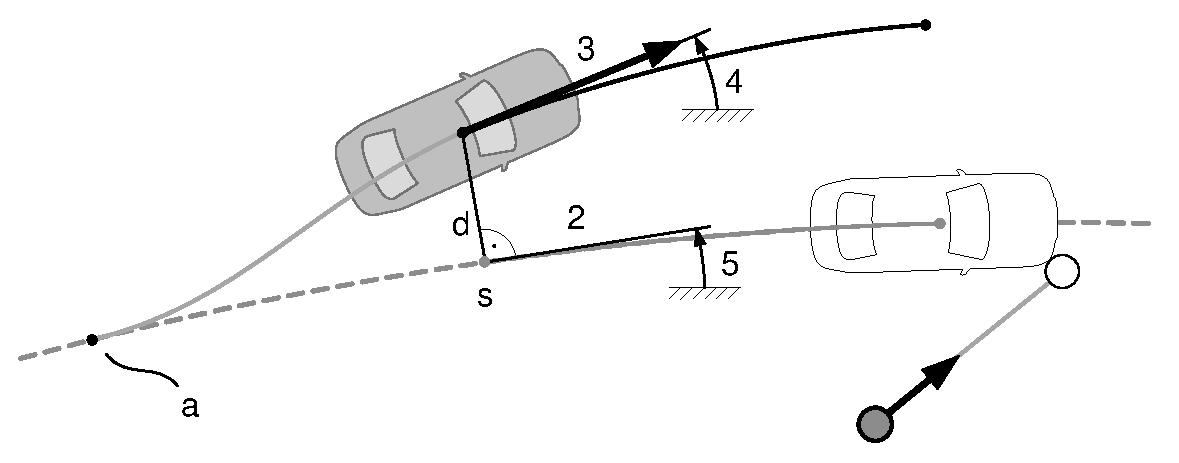
\includegraphics[width=.8\textwidth,clip, trim = 0cm 0cm 0cm 0cm]{6_Draufsicht_Zustaende.eps}
    \caption[Prädizierte Fahrkurve und Optimaltrajektorie]{Prädizierte manuelle Fahrkurve (grau-gestrichelt) zum Aktivierungszeitpunkt mit vorausberechnetem Kollisionspunkt (weißes Fahrzeug, weißer Fußgängerkreis), Historie der Ausweichtrajektorie (grau), aktuelle Fahrzeug- und Hindernisposition (graues Fahrzeug, grauer Fußgängerkreis) und Optimaltrajektorie (schwarz) zum Ausweichen \citeltex{werling2014riccati}}
    \label{fig:Draufsicht_Zustaende}
\end{figure}
%
Die Systemmodellierung gestaltet sich mit Zustand $\bs x^\T = [x_1, x_2, x_3] = [d_r\!-\! o, \dot d_r, \ddot d_r]$ und (virtuellem) Eingang $u=\dddot d_r$ dementsprechend einfach:
\begin{align} \label{ric_systemdyn}
		\dot{\bs x} = \mmatrix A \bs x + \bs b u, \quad \bs x(t_0) = \bs x_0,
\end{align}
\[
\mmatrix A= \left[ \begin{array}{ccc} 0& 1& 0\\ 0&0&1\\ 0&0&0\end{array} \right], \quad
%\quad \text{und} \quad 
\bs b= \left[ \begin{array}{c} 0\\ 0\\ 1\end{array} \right]
\]
Die Variable $o$ beschreibt hierbei die prädizierte Überlappung des Fahrzeugs mit dem um einen Sicherheitsabstand vergrößerten Hindernis zum vermeintlichen Kollisionszeitpunkt, s.\ Bild~\ref{fig:Lokale_Koordinate_Ausweichen}, und wird später in \eqref{equ:xi_1} quantifiziert. Da sich die manuelle Referenzkurve entsprechend über den Fahrzustand zum Aktivierungszeitpunkt $t_0$ definiert, gilt somit $\bs x^\T_0 = [-o, 0, 0]$, s.\ Bild~\ref{fig:Lokale_Koordinate_Ausweichen}.

Ziel ist es nun, den Systemeingang $u$ in jedem Zeitschritt $t_k$ so zu optimieren, dass das Fahrzeug bis zum Zeitpunkt $t_1$ keine Überlappung mehr mit dem Hindernis aufweist, dieses also sicher passiert, und bis zum Zeitpunkt $t_f$ wieder entlang der manuellen Referenz ausgerichtet ist.  

\begin{figure}[h]
\centering
	\psfrag{0}[tc][tc]{$t_0$}
	\psfrag{1}[tc][tc]{$t_1$}
	\psfrag{2}[tc][tc]{$t_f$}
	\psfrag{3}[cr][cr]{$0$}
	\psfrag{o}[cr][cr]{$-o$}
	\psfrag{x}[cr][cr]{$x_1$}
	\psfrag{t}[cc][cc]{$t_k$}
	\centering
  	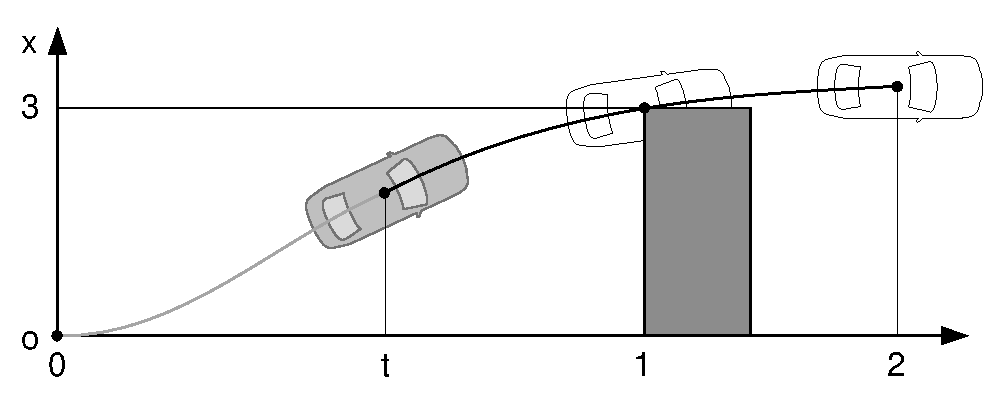
\includegraphics[width=1.\textwidth,clip, trim = 0cm 0cm 0cm 0cm]{6_Lokale_Koordinate_Ausweichen.eps}
  \caption[Ausweichvorgang in den Koordinaten der Ursprungskurve]{Ausweichvorgang in den Koordinaten der manuellen Ursprungskurve mit erforderlicher Versatzbreite (graues Rechteck) und Endzustand \citeltex{werling2014riccati}}
    \label{fig:Lokale_Koordinate_Ausweichen}
\end{figure}

%\subsubsection{Kostendefinition}
Mit Hilfe des Zustandsvektors $\bs x$ und der Systemstellgröße $u$ lässt sich nun das Kostenfunktional 
\begin{align}
		J = \int\limits_{t_k}^{t_f} l(\bs x(t),u(t)) {\rm d} t + \tilde V(\bs x(t_1), \bs x(t_f)) \label{equ:gesamtkosten}
\end{align}
definieren, welches neben den Integralkosten $l$ jetzt auch die Punktkosten $\tilde V$ beinhaltet. Erstere sind gegeben durch %die quadratischen Integralkosten% $l(x(t),u(t))$
\begin{align*}
l(\bs x(t),u(t)) &= \frac{1}{2} \left[ \bs x(t)^\T \bs Q \bs x(t) + r u^2(t) \right], \\
\bs Q &= \text{diag}(0, q_2, q_3), \quad r := 1.
\end{align*}
Da $x_2$ die Ableitung $\dot d_r$ darstellt, bestraft $q_2>0$ hierbei die quadratische Versatzgeschwindigkeit. Aufgrund des Integrals in \eqref{equ:gesamtkosten} werden damit kleine Versatzbreiten für den gesamten Ausweichvorgang bevorzugt. Die Kostenparameter $q_3>0$ und $r:=1$ wiederum führen zu einer Vermeidung großer Versatzbeschleunigungsquadrate $(\ddot d_r)^2$ und -ruckquadrate $(\dddot d_r)^2$, sodass die Fahrphysik und die Fahrzeuginsassen nicht unnötig strapaziert werden. \\
Anstelle "`harter"' Nebenbedingungen an die Trajektorie wird das gewünschte Verhalten am internen Randpunkt $t_1$ und am Endpunkt $t_f$ über quadratische Punktkosten $\tilde V(\bs x(t_1), \bs x(t_f))$ 
%Dadurch können Singularitäten vermieden werden, welche in der Praxis mit Nebenbedingungen in der Online-Optimierung einher gehen.\footnote{Wird in der zyklischen Optimierung die Einhaltung von Gleichungs- oder Ungleichungsrestriktion gefordert, steigt die Rauschanfälligkeit des Systems an, je näher es der (aktiven) Restriktion kommt, da diese unter allen Umständen eingehalten werden muss. Für viele Problemstellungen ist allerdings keine absolute Genauigkeit erforderlich. Ein Ausweg ist dann eine Problemformulierung, welche die Verletzung der Nebenbedingungen lediglich mit hohen Kosten bestraft \cite{Findeisen2002}.} %sog.\ barrier-functions dar, mit entsprechend hohen Wichtungsfaktoren}. 
der Form
\begin{align}	\label{equ:punktkosten}	
		&\tilde V(\bs x_1, \bs x_f) = \frac{1}{2} \left[ \bs x_1^\T \bs S_1 \bs x_1 + \bs x_f^\T \bs S_f \bs x_f\right], \\
		&\bs S_1 = \text{diag}(s_{11}, 0, 0), \quad \bs S_f = \text{diag}(0, s_{22}, s_{33}),
\end{align}
mit $\bs x_1 = \bs x(t_1)$ und $\bs x_f = \bs x(t_f)$ herbeigeführt. Ein großes $s_{11}>0$ stellt sicher, dass das Fahrzeug das Hindernis möglichst genau mit dem vorgegebenen Sicherheitsabstand passiert (\,$x_1(t_1) \approx 0$\,); am Manöverende hingegen erzwingen große $s_{22}>0$ und $s_{33}>0$, dass das Fahrzeug keine merkliche Relativgeschwindigkeit und -beschleunigung zur manuellen Ursprungskurve mehr aufweist. Die Endposition wird nicht vorgeschrieben, damit das Fahrzeug nicht wieder hinter dem Hindernis einschert, wofür keine verlässliche Sensorinformation verfügbar ist und wo sich das nächste Hindernis befinden kann.


%\begin{align*}
		%J = \tilde V[d_r(t)] + \int\limits_{t_0}^{t_{1}} l[d_r(t)] \, {\rm d} t
%\end{align*}
%realisieren, welches sich aus Integralkosten $l$ und Punktkosten $\tilde V$ zusammensetzt. Die Integralkosten sind hierbei definiert als
%\begin{align*}
		%l:= k_1 (\dot d_r)^2 + k_2 (\ddot d_r)^2 + k_3 (\dddot d_r)^2,
%\end{align*}
%wobei $d_r(t)$ den Abstand des Fahrzeugs von der prädizierten Fahrkurve beschreibt, welche sich ohne Eingriff ergeben hätte, s.\ Bild~\ref{fig:Draufsicht_Zustaende}.
%




%Durch die Vereinfachung der Fahrzeugdynamik auf die Querdynamik bezüglich einer Referenzkurve kann die Fahrzeugbewegung in Querrichtung durch das lineare dynamische System 
%\begin{align} \label{ric_systemdyn}
		%\dot x = A x + B u, \quad x(t_0) = x_0
%\end{align}
%mit den Systemmatrizen
%\[
%A= \left( \begin{array}{ccc} 0& 1& 0\\ 0&0&1\\ 0&0&0\end{array} \right)
%\quad \text{und} \quad 
%B= \left( \begin{array}{c} 0\\ 0\\ 1\end{array} \right)  \hspace{1.0cm}
%\]
%beschrieben werden. 
%Wie bereits erwähnt ist es für ein autonomes Ausweichmanöver nur sinnvoll, eine optimale Regelung über einen endlichen Zeithorizont zu berechnen, womit sich das Kostenfunktional in der folgenden Form darstellen lässt:
%\begin{align*}
		%J = \tilde V(x_s, x_e) + \int\limits_{t_0}^{t_{\text{end}}} l(x(t),u(t)) {\rm d} t.
%\end{align*}
%Hierbei beschreiben die quadratischen Integralkosten% $l(x(t),u(t))$
%\begin{align*}
%l(x(t),u(t)) = & \frac{1}{2} \left[ x(t)^\T Q x(t) + u(t)^\T R u(t) \right]
%\end{align*}
%einen Strafterm während des Ausweichmanövers, wohingegen die Punktbedingung $\tilde V(x_s, x_e)$ die Trajektorienkosten zu den Zeitpunkten $t_s$ und $t_e$ beschreibt. 

\subsection{Lösung des Optimalsteuerungsproblems}\index{Optimalsteuerung} \label{sec:problemloesung}
%Um ein gezieltes Ausweichen zu ermöglichen, ist im Speziellen der Zustand der Trajektorie neben dem Hindernis (zum Zeitpunkt $t_s$) und zum Endzeitpunkt $t_e$, an dem der Ausweichvorgang beendet wird, interessant. Hierzu definiert man zusätzlich die quadratischen Punktkosten
%\begin{align*}		
		%\tilde V(x_s, x_e) = & \frac{1}{2} \left[ x_s^\T S_s x_s + x_e^\T S_e x_e\right].
%\end{align*}

%Im Hinblick auf die Ergebnisse aus Abschn.\,\ref{sec:riccati_dgl} fehlen für die beiden Teilintervalle $[t_0,t_1)$ und $[t_1,t_f]$ nur noch die Anfangsbedingungen für $\bs P(t)$ in \eqref{equ:riccati-diffgl}.
Wie bereits in Abschn.\,\ref{sec:riccati_dgl} folgt aus \eqref{equ:trans_x_frei} unmittelbar für $t_f$ die Endbedingung
\begin{align} \label{equ:endbedingungen}
\bs P(t_f) = \bs S_f \;,
\end{align}
s.\ Gleichung~\eqref{equ:endbedingungen_orig}.
%wie bereits in \eqref{equ:riccati_randwerte} dargestellt. 
Im Unterschied dazu teilt nun der interne Randpunkt in $t_1$ den Optimierungshorizont in zwei Teilintervalle $[t_0,t_1)$ und $[t_1,t_f]$. Die Lösung der Differentialgleichung \eqref{equ:riccati-diffgl} für $\bs P(t)$ erfordert demnach eine weitere Anfangsbedingung, 
%Aufgrund der Punktkosten auf Höhe des Hindernisses, also zum Zeitpunkt $t_1$, ist nun die Herleitung der klassischen LQ-Regelung mit endlichem Optimierungshorizont anzupassen. 
%So wie in \eqref{equ:F} durch Modifikation der Integralkosten mittels Lagrange-Multiplikator $\bs \lambda(t)$ die Differentialgleichung Berücksichtigung findet, wird im Folgenden durch Erweiterung der Punktkosten \eqref{equ:punktkosten} zu
%\begin{align} \label{equ:mod_pktkosten}
%\tilde V_\sigma(\bs x_1^-, \bs x_1^+, \bs x_f)& := \tilde V(\bs x_1^-, \bs x_f) + \bs \sigma^\T[\bs x_1^- - \bs x_1^+]
%\end{align}
%die Stetigkeit der Systemtrajektorie in $t_1$, also $\bs x_1^- = \bs x_1^+$, über einen zusätzlichen Lagrange-Multiplikator $\vektor \sigma$ sichergestellt. Hierbei beschreiben $\bs x_1^-$ und  $\bs x_1^+$ den Systemzustand $\bs x_1$ unmittelbar vor und nach dem Zeitpunkt $t_1$; die Schreibweise wird nachfolgend auf weitere Variablen angewandt.
%Unter Zuhilfenahme der Funktion 
%\begin{align}
%	F(\bs x,u)& = l(\bs x,u) + \bs \lambda^T(\bs A \bs x+\bs b u-\dot{\bs x}) \label{equ:F}
%\end{align}
die sich aus der Transversalitätsbedingung \eqref{equ:interne_randpunkte_lambda} zu
\begin{align*}
\frac{\partial \tilde  V}{\partial\bs x_1}-\bs \lambda(t_1^-) + \bs \lambda(t_1^+) &= \bs 0
%\left(\frac{\partial \tilde  V_\sigma}{\partial\bs x_1^-}+\frac{\partial F^-}{\partial \dot{\bs x}}\right)_{t_1}  &= 0 \\
%\left(\frac{\partial \tilde  V_\sigma}{\partial \bs x_1^+}-\frac{\partial F^+}{\partial \dot{\bs x}}\right)_{t_1} &= 0 \\
%\left(\frac{\partial \tilde  V_\sigma}{\partial \bs x_f}-\frac{\partial F}{\partial \dot{\bs x}}\right)_{t_f} &= 0 \; .
\end{align*}
ergibt.
%Während sich mit \eqref{equ:adjungierteDGL} aus der letzen Gleichung durch Koeffizientenvergleich unmittelbar für $t_f$ die \emph{Endbedingung} 
%\begin{align} \label{equ:endbedingungen}
%\bs P(t_f) = \bs S_f
%\end{align}
%ergibt, folgt aus den ersten beiden zunächst
%\begin{align*}
%\bs S_1 \bs x_1^- + \bs\sigma - \bs\lambda^-(t_1) &\Rightarrow \bs\lambda^-(t_1) = \bs S_1 \bs x_1^- + \bs\sigma\\
%- \bs\sigma + \bs\lambda^+(t_1) &\Rightarrow \bs\lambda^+(t_1) = \bs\sigma \; .
%\end{align*}
%Mit $\bs x_1=\bs x_1^-=\bs x_1^+$ und \eqref{equ:adjungierteDGL} kann $\bs \sigma$ eliminiert werden, sodass sich für $t_1$ schließlich die \textit{Punktbedingung}
Mit \eqref{equ:riccati_ansatz} wird nämlich $\,\bs S \bs x_1 - \bs P(t_1^-) \bs x_1 + \bs P(t_1^+) \bs x_1 = \bs 0$ erhalten und damit gilt
\begin{align*} 
\bs P(t_1^-)= \bs P(t_1^+) + \bs S_1 \;. % \label{riccati-pktbed-sprung}
\end{align*}
Mit anderen Worten:  $\bs P(t)$ springt zum Zeitpunkt $t_1$ um die internen Punktkosten $\bs S_1$ und entspricht am Ende der Trajektorie den Endkosten $\bs S_f$.
%
%In den Zeitpunkten $t_1$ und $t_f$ müssen zusätzlich die notwendigen \textit{Transversalitätsbedingungen}, d.\,h.
%\begin{align} \!\!\!\!\!\!\!
	%\left(\frac{\partial \tilde V}{\partial x_1}+F_{\dot{x}}\right)_{t_1} = 0 \quad \text{und}
	%\quad \left(\frac{\partial \tilde V}{\partial x_2}+F_{\dot{x}}\right)_{t_f} = 0\, ,
%\end{align}
%erfüllt werden. Wird in diese Gleichungen $F(\bs x,u)$ und $\tilde V(\bs x_1, \bs x_f)$ eingesetzt, so ergeben sich durch Koeffizientenvergleich
%\begin{align*}
%P(t_1) = S_1 \quad \text{und}
	%\quad P(t_f) = S_f \;.
%\end{align*}
%Bis zu dieser Stelle wurden die beiden Abschnitte... [hier weiter: oben erst $\tilde \tilde V$ definieren, dann weiterrechnen.]
%
%Mit der Matrix-Riccati-Differentialgleichung \eqref{equ:riccati-diffgl}, dem Stellgesetz \eqref{equ:stellgesetz} und den beiden obigen Punktbedingungen ist es möglich einen schaltenden Regler zu implementieren. Dieser Regler betrachtet jedoch beide Zeitintervalle unabhängig voneinander und berechnet somit keine optimale Lösung über das gesamte Zeitintervall. Um dies zu erreichen, ist eine Abänderung des Systemmodells notwendig.
%
%Hierzu lässt man (theoretisch) einen Sprung des Systemzustandes x zum Zeitpunkt $t_s$ zu, bestraft diesen Sprung jedoch durch folgende Modifikation des Punktkosten:
%\begin{align} \label{equ:mod_pktkosten}
%\tilde \tilde V(\bs x_1^-, \bs x_1^+, \bs x_f)& := \tilde V(\bs x_1^-, \bs x_f) + \bs \sigma^\T[\bs x_1^- - \bs x_1^+]
%\end{align}
%Durch diese Modifikation folgen aus der Optimalsteuerung aus der ersten Variation zwei weitere Nebenbedingung an die optimale Trajektorie:
%\begin{align*}
%\left(\frac{\partial \tilde \tilde V}{\partial\bs x_1^-}+\frac{\partial F^-}{\partial \dot{\bs x}}\right)  = 0 \\
%\left(\frac{\partial \tilde \tilde V}{\partial \bs x_1^+}-\frac{\partial F^-}{\partial \dot{\bs x}}\right) = 0
%\end{align*}
%Aus diesen Koppelbedingungen folgt wiederum:
%\begin{align*}
%S_1\cdot \bs x_1^- + \bs\sigma - \bs\lambda^-(t_1) &\Rightarrow \bs\lambda^-(t_1) = S_1\cdot \vector x_1^- + \bs\sigma\\
%- \bs\sigma + \bs\lambda^+(t_1) &\Rightarrow \bs\lambda^+(t_1) = \bs\sigma
%\end{align*}
%Da die Stetigkeit des Systemzustand jedoch notwendig ist, gilt mit $\bs x_1=\bs x_1^-=\bs x_1^+$ und \mbox{$\bs\lambda(t) = P(t) \cdot \bs x(t)$} die \textit{Punktbedingung}:
%\begin{align} 
%P^-(t_1)= P^+(t_1) + S_1 \label{riccati-pktbed-sprung}
%\end{align}
%Diese Punktbedingung koppelt die beiden Phasen des schaltenden Reglers und regelt das System auf ein optimale Lösung bzgl. des vollständigen Zeitinvervalls ein.
%
%Mit der Punktbedingungen  \eqref{equ:endbedingungen} und \eqref{riccati-pktbed-sprung} sowie der Matrix-Riccati-Differentialgleichung \eqref{equ:riccati-diffgl} 
Damit lässt sich durch Rückwärtsintegration die matrixwertige Funktion $\bs P(t)$ für $t\in\left[t_0,t_f\right]$ numerisch berechnen, was genauer im nächsten Abschnitt beschrieben wird. \\
Zuvor muss jedoch noch ein Sonderfall behandelt werden, der vor allem beim aktiven Mitlenken des Fahrers zum Tragen kommt. Das Optimierungsziel in \eqref{equ:punktkosten} ist nämlich, dass das Fahrzeug zum Zeitpunkt $t_1$ möglichst genau den seitlichen Sicherheitsabstand zum Hindernis einhält. Lenkt jetzt der Fahrer eigenständig mit größerem Sicherheitsabstand als parametriert am Hindernis vorbei, versetzt eine Störung das Fahrzeug etwas weiter vom Hindernis weg als zunächst geplant oder zieht sich die Prädiktion des Hindernisses aus dem Fahrschlauch zurück (z.B. weil der Fußgänger stehenbleibt), dann würden die Punktkosten \eqref{equ:punktkosten} dazu führen, dass das Fahrzeug wieder zum Hindernis "`hingezogen"' wird. Um das zu verhindern, muss eine einfache Fallunterscheidung durchgeführt werden: Führt die Trajektorie unter Berücksichtigung des links (rechts) zu passierenden Hindernisses zu einem größeren (kleineren) Ruck $u$ als ohne Hindernis, dann ist der Ausweichtrajektorie zu folgen. Andernfalls ist das Hindernis im aktuellen Zeitschritt zu ignorieren und die Stellgröße der Optimierung ohne Hindernis zu verwenden. \\
Die Trajektorie ohne Hindernis kann hierbei wie die im Folgenden beschriebene Trajektorie mit Hindernis generiert werden, indem lediglich die Punktkosten für $t_1$ der Nullmatrix gleichgesetzt werden, d.h.\
\begin{align*}
	\tilde{ \bs S}_1 = \bs 0 \; ,%\\
	%u = \max()
\end{align*}
und das klassische LQ-Problem mit endlichem Optimierungshorizont gelöst wird.

%[Für die Praxistauglichkeit des Regler bleibt noch ein weiterer Sonderfall zu beachten: Im Falle einer Falschauslösung würde durch das quadratische Kostenfunktional das Fahrzeug durch die Bestrafung des Abstands in der Position unnötig an das Hindernis herangeregelt werden. Um dieses Problem zu umgehen wird ein zweiter Satz an Matrizen $\tilde P(t)$ berechnet, der sich dadurch unterscheidet, dass die Punktkostenmatrix $S_1$ für diese Matrizen gleich der Nullmatrix entspricht. Zur Laufzeit werden nun beide Stellgrößen über das Stellgesetz \eqref{equ:stellgesetz} berechnet und die größere Stellgröße an den unterlagerten Regler weitergegeben.]


%Inaktive Punktkosten (ehem. freespace)

%Die übrigen Matrizen haben dabei folgende Form: 
%\begin{align*}
	%Q &= \diag{0, q_v, q_a} \\
	%R &= 1 \\
	%S_1 &= \diag{s_1, 0, 0} \\
	%S_f &= \diag{0, s_{ev}, s_{ea}},
%\end{align*}
%wobei die Variablen $q_v, q_a, s_1, s_{ev}$ und $s_{ea}$ geeignet zu wählen sind.
%
%Endbedingung
%\begin{align*} %\label{}
%P(t_f) = S_f
%\end{align*}
%
%Punktbedingung
%\begin{align} \label{riccati-pktbed-sprung}
%P^-(t_1)= P^+(t_1) + S_1
%\end{align}

%\subsection{Implementierung} \label{sec:implementierung}
\subsection{Rückwärtsintegration und Zeittransformation} \label{sec:rueckwaertsintegration}
\begin{table}[t]
\centering
\begin{tabular}{p{\columnwidth}}
\hline \\
\textbf{1) Parametrierung}
\begin{itemize}
\item Wahl der Kostenwichtungsfaktoren $q_2, q_3, s_{11}, s_{22}, s_{33}$
\item Festlegung der Zeitpunkte $t_0, t_1, t_f$
 %$T_\text{tc}_\text{max}, T_\text{tc}_\text{min}$
%\item $\Rightarrow t_1 = T_\text{tc}_\text{max}, t_f = T_\text{tc}_\text{max}-T_\text{tc}_\text{min}$
\end{itemize}
\\

\textbf{2) Rückwärtsintegration bis zum Hindernis} \\ 
\quad DGL \eqref{equ:riccati-diffgl} mit $\bs P(t_f) = \bs S_f, \quad \tau \in [t_1, t_f]$
\\
\\

%\begin{itemize}
%\item DGL \eqref{equ:riccati-diffgl} mit $P(t_f) = S_f, \quad \tau \in [t_1, t_f]$
%\item $\tilde P(\tau) = P(\tau)$
%\end{itemize} 
%\\

\textbf{3) Rückwärtsintegration ab Hindernis} \\ 
\quad DGL \eqref{equ:riccati-diffgl} mit $\bs P(t_1^-)= \bs P(t_1^+) + \bs S_1, \quad \tau \in [t_0, t_1)$
\\
\\

\textbf{4) Berechnung der Verstärkungsmatrix} \\
%\begin{itemize}
\quad $\bs K(\tau) = r^{-1} \bs b^\T \bs P(\tau), \quad \tau \in [t_0, t_f]$
\\
\\

%\item $\tilde K(\tau) = R^{-1} B^\T \tilde P(\tau)$ 
%\end{itemize}
%\\
\hline \\
\end{tabular}
\caption{Berechnungen der $\bs K$-Matrix des LQ-Optimierungsproblems}
\label{tab:bestimmungKMatrix}
\end{table}
Wie bereits im vorhergehenden Abschnitt erwähnt, kann $\bs P(t)$ durch numerische Rückwärtsintegration\footnote{Zur Verwendung von Standard-DGL-Solvern muss das matrixwertige Differentialgleichungssystem \eqref{equ:riccati-diffgl} in ein vektorwertiges umgeschrieben und der rückwärtslaufenden Zeit Rechnung getragen werden.} gelöst werden. Entsprechend Tabelle~\ref{tab:bestimmungKMatrix} wird hierbei ausgehend von den Endkosten zum Zeitpunkt $t_f$ die Riccati-Differentialgleichung \eqref{equ:riccati-diffgl} rückwärts integriert. Zum Zeitpunkt $t_1$ werden dann die Punktkosten hinzuaddiert bis schließlich $t_0$ erreicht wird. Für das Stellgesetz \eqref{equ:stellgesetz} kann daraus direkt die $\bs K$(t)-Matrix bestimmt werden.

Diese Berechnung stellt keinen übermäßigen Rechenaufwand dar, der ein Lösen zur Laufzeit verbietet, \vgl \cite{Graichen2012, Buskens09}. % Buskens09: Änderung des Optimierungsproblems }.
Jedoch kann bei festem $t_{12}:=t_f - t_1$, also der Stabilisierungszeit zwischen Passieren des Hindernisses und der Übergabe an den Fahrer, die $\bs K(t)$-Matrix durch eine geeignete Zeittransformation vorberechnet werden, sodass sich der Online-Rechenaufwand auf den eines gewöhnlichen Zustandsreglers reduziert. \\
Hierzu wird die bereits in Abschn.\,\ref{sec:ttc} eingeführte time-to-collision\index{time-to-collision} $T_\text{tc}$ herangezogen. Da es aufgrund des Ausweichmanövers zu keiner Kollision kommt, beziffert sie hier die verbleibende Zeit des auf die ursprüngliche Referenzkurve projizierten Fahrzeugs bis es das Hindernis berührt, s.\ Abb.\,\ref{fig:Draufsicht_Zustaende}. Mit dem vermeintlichen Kollisionszeitpunkt $t_1$ ergibt sich somit
\begin{align*}
	T_\text{tc} := t_1-t_k \; .  %\label{equ:TTC2t}
\end{align*}
Die Vorberechnung der Matrix $\bs K(T_\text{tc})$ muss jetzt lediglich für den Bereich zwischen $T_\text{tc} = t_1-t_f$, also dem für alle Ausweichmanöver gemeinsamen Übergabezeitpunkt an den Fahrer nach der vermiedenen Kollision, und einer $T_\text{tc}$, oberhalb derer überhaupt keine Auslösung der Funktion in der Praxis mehr auftritt, analog Tabelle~\ref{tab:bestimmungKMatrix} durchgeführt werden.

\subsection{Zustandstransformation für unterlagerte Folgeregelung}
Um auf eine absolute Eigenlokalisierung zu verzichten, etwa über GPS oder Landmarken, % Aufgrund einer fehlenden verlässlichen Absolutposition und -ausrichtung wie differentielles GPS in Serienfahrzeugen ist 
kann nach Aktivierung des Systems in jedem Schritt die Position und Bewegungsrichtung des Fahrzeugs durch Koppelnavigation\index{Koppelnavigation}, s.\ Abschn.\,\ref{sec:koppelnavi} näherungsweise bestimmt werden. Anschließend müssen dann der Abstand und die Ausrichtung zur Referenzkurve errechnet werden. Wird hierfür direkt die Relativbewegung
\begin{subequations} \label{equ:relativbewegung}
\begin{align} 
	\!\!\!\!\!\! \dot d_r      &= v \sin\Delta\theta, &d_r(t_0) = 0 \label{equ:dgl_d_r_dot} \\
	\!\!\!\!\!\! \Delta\dot\theta &= v \left[\kappa  - \frac{\cos\Delta\theta}{1 - d_r \kappa_r} \kappa_r\right], &\Delta\theta(t_0) = 0 \label{equ:theta_r_dot} 
\end{align}
\end{subequations}
vom Fahrzeug zur Referenzkurve, s.\ z.B.\ \cite{werivcontrol08}, mit Differenzkurswinkel $\Delta\theta = \theta-\theta_r$ und Fahrgeschwindigkeit $v$ herangezogen, erfolgt das in einem Schritt. Hierzu ist eine Schätzung der Kurskrümmung $\kappa(t)$ des Fahrzeugs mittels der ESP-Serieninertialsensorik erforderlich. Die geschätzte Istkrümmung wird auch zum Zeitpunkt der Aktivierung $t_0$ für die Referenzkurve übernommen, d.h.\ $\kappa_r = \kappa(t_0) = \text{const.}$, s.\ Abb.\,\ref{fig:Draufsicht_Zustaende}.

Die Transformation in den Systemzustand $\bs x^\T = [x_1, x_2, x_3]$ der Optimierung ist dann gegeben durch
\begin{subequations} \label{equ:lin_stat_trafo}
\begin{align}
	x_1 &= d_r - (\underbrace{ d_\text{obs} + d_s + \tfrac{1}{2}( b + b_\text{obs} )}_{:= o})\label{equ:xi_1}
	\\
	x_2 &= \dot d_r = v  \sin\Delta\theta \label{equ:xi_2} \\
\nonumber
	x_3 &= \ddot d_r = v \cos\Delta\theta \cdot \Delta\dot\theta + \dot v \sin\Delta\theta \\
	&=  v^2 \cos\Delta\theta\left[\kappa  - \frac{\cos\Delta\theta}{1 - d_r \kappa_r} \kappa_r\right] + a \sin\Delta\theta \label{equ:xi_3}
\end{align}
\end{subequations}
wobei $d_\text{obs}$ die Querposition des Hindernisses zur Referenzkurve zum vermeintlichen Kollisionszeitpunkt, $d_s$ den  Sicherheitsabstand und $b$ bzw.\ $b_\text{obs}$ die Breite des Eigenfahrzeugs und des Hindernisses bezeichnen. Die Fahrzeugbeschleunigung in Bewegungsrichtung ist wiederum gegeben durch $a = \dot v$.

In der Praxis hat sich die asymptotische Stabilisierung der Fahrkrümmung $\kappa$ durch einen unterlagerten Lenk\-reg\-ler bewährt, s.\ Abschn.\,\ref{sec:asymptotische_folgeregelung}.  Damit das hierzu notwendige Referenzsignal $\kappa_d(t)$ stetig verläuft, wird zunächst ein $x_{3,d}$ durch Integration der virtuellen, optimierten Stellgröße $u^\ast$ bestimmt, d.h.\
%
%Da $x_3$ hier mit einem Folgeregler asymptotisch stabilisiert wird, darf dieser Zustand nicht rückgeführt werden, da so die Regelabweichung zu null gesetzt werden würde und nur noch die Vorsteuerung der unterlagerten Folgeregelung aktiv wäre. Stattdessen ist ein $x_{3,d}$ durch Integration von $u$ zu bestimmen, d.h.\
\begin{align}
\nonumber
	\dot x_{3,d} &= u^\ast \; , \quad x_{3,d}(t_0) =  0 \; ,
\end{align}
und der Optimierung selbst wiederum als Systemzustand $x_3 = x_{3,d}$ zurückgeführt, vgl.\ auch Abb.\,\ref{fig:KR_Integrator_Erweiterung} auf S.\,\pageref{fig:KR_Integrator_Erweiterung}. %Ferner muss das Referenzsignal $x_{3,d}$ in eine Krümmungsreferenz umgerechnet werden. %Hierzu wird \eqref{equ:dgl_d_r_dot} abgeleitet und mit $a(t) = \dot v(t)$ der Zusammenhang TODO
%\begin{align*}
	%x_3 &= \ddot d_r = v(t) \cos\Delta\theta \cdot \Delta\dot\theta + a(t) \sin\Delta\theta
	%\end{align*}
%erhalten.
%
%
Mit $\kappa = \kappa_d$ und \eqref{equ:xi_3} wird nach Auflösen dann sofort die umzusetzende Referenzkrümmung
\begin{align}	\kappa_d &= \frac{x_{3,d} - a \sin  \Delta\theta}{v^2 \cos  \Delta\theta} + \frac{\cos \Delta\theta}{1-d_r \kappa_r}\kappa_r \; . \label{equ:kappa_d}
\end{align}
erhalten. 
%was als Krümmungssollvorgabe an die unterlagerte Folgeregelung weitergeleitet wird.
Der Gesamtablauf des Algorithmus kann Abb.\,\ref{fig:RiccatiAblauf} entnommen werden.

 

% Hinweis für Habil: wenn gute schwimmwinkelschätzung vorhanden, dann sollte dot psi = r separat integriert werden, da die summe theta = psi + beta dann genauer als wenn auch das verrauschte dotbeta mit interiert wird. Hier allerdings wird von überhaupt keinem fahrzeugmodell ausgegangen, da nur sehr kurz integriert wird und damit der schwimmwinkel auch nur aus querbeschleunigung und gierrate integriert wird
%Koppelnavigation
%\begin{align*} %\label{}
	%\theta(t) 			&= \psi(t) + \beta(t) \\
	%\kappa(t)       &= \frac{1}{v}\dot\theta = \frac{1}{v}[r + \dot \beta] \\
	%\dot\psi 	&= r, \quad \psi(t_0) = 0
%\end{align*}
%Schwimmwinkel $\beta$ und Schwimmwinkeländerung $\dot\beta$ wird geschätzt, Gierrate integriert


\begin{figure}
\centering
	\psfrag{A}[cr][cr]{$\begin{bmatrix} \kappa \\ v \end{bmatrix}$}
	\psfrag{a}[cl][cl]{$$}
	\psfrag{B}[cl][cl]{$x_3$}
	%\psfrag{Y}[cl][cl]{$\kappa_0$}
	\psfrag{T}[cl][cl]{$T_\text{tc}$}
	\psfrag{O}[cr][cr]{$d_\text{obs}$}
	
	\psfrag{5}[cc][cc]{\eqref{equ:relativbewegung}}%{\eqref{equ:dgl_d_r_dot},\eqref{equ:theta_r_dot}}
	\psfrag{0}[cl][cl]{\parbox[t]{4cm}{Fahrzeugrelativbewegung \\ zur Referenzkurve}}
	%
	\psfrag{C}[cl][cl]{$[d_r, \Delta\theta]$} % kappa_r
	\psfrag{4}[cc][cc]{\eqref{equ:xi_1},\eqref{equ:xi_2}}
	\psfrag{9}[cl][cl]{\parbox[t]{3cm}{Linearisierende\\Zustandstransformation} }
	%
	\psfrag{D}[cl][cl]{$[x_1, x_2]$}
	\psfrag{3}[cc][cc]{\eqref{equ:stellgesetz}} %\eqref{equ:TTC2t},
	\psfrag{8}[cl][cl]{\parbox[t]{4cm}{Linear-quadratische \\ Trajektoriengenerierung}}
	%
	\psfrag{E}[cl][cl]{$u^\ast$}
	\psfrag{i}[cc][cc]{$\int$}
	%
	\psfrag{F}[cl][cl]{$x_{3,d}$}
	\psfrag{2}[cc][cc]{\eqref{equ:kappa_d}}
	\psfrag{7}[cl][cl]{Rücktransformation}
	\psfrag{G}[cl][cl]{$\kappa_{d}$}
	%
	\psfrag{\tilde V}[cl][cl]{$\kappa_d$}
	\psfrag{1}[cc][cc]{\zB \cite{urmson2008adu}}%\eqref{equ:theta_dot}}
	\psfrag{6}[cl][cl]{\parbox[t]{4cm}{Krümmungsregelung \\ und Fahrzeugdynamik}}
	%
	\psfrag{n}[lb][lb]{$[d_r,\!\Delta\theta]$}
	\psfrag{m}[lb][lb]{$[v,a]$}
	\centering
  	\includegraphics[width=.75\textwidth,clip, trim = 0cm 0cm 0cm 0cm]{6_LQR_Ablauf.eps}
  \caption[Aufbau der Riccati-basierten Trajektorienplanung]{Aufbau der Riccati-basierten Trajektorienplanung \citeltex{werling2014riccati}}
  \label{fig:RiccatiAblauf}
\end{figure}


\subsection{Implementierung und Evaluation im Realversuch}\label{sec:eval}

%\subsection{Evaluation des Gesamtsystems}
%
%\subsubsection{Prototypische Umsetzung}
Für den Funktionsnachweis wurden %die Steuergerätesoftware der Serienservolenkung einer BMW 5er Limousine der sechsten Generation modifiziert, sodass sie als Aktor zur Verfügung steht. Des Weiteren sind 
die Algorithmen der Trajektorienoptimierung und Krümmungsregelung in Simulink/Embedded Matlab implementiert. Sie laufen auf einer dSpace Autobox 
mit einer Zykluszeit von $\unit[10]{ms}$, von der die für die Optimierung erforderlichen Rechenoperationen nur einen Bruchteil beanspruchen. Die Fußgängerdetektion und -klassifikation erfolgt über Kamera, s.\ schwarzer Kasten rechts neben dem Rückspiegel in Abb.\,\ref{fig:Innenansicht_Fahrzeug}.

\begin{figure}[!ht]
	\centering
  	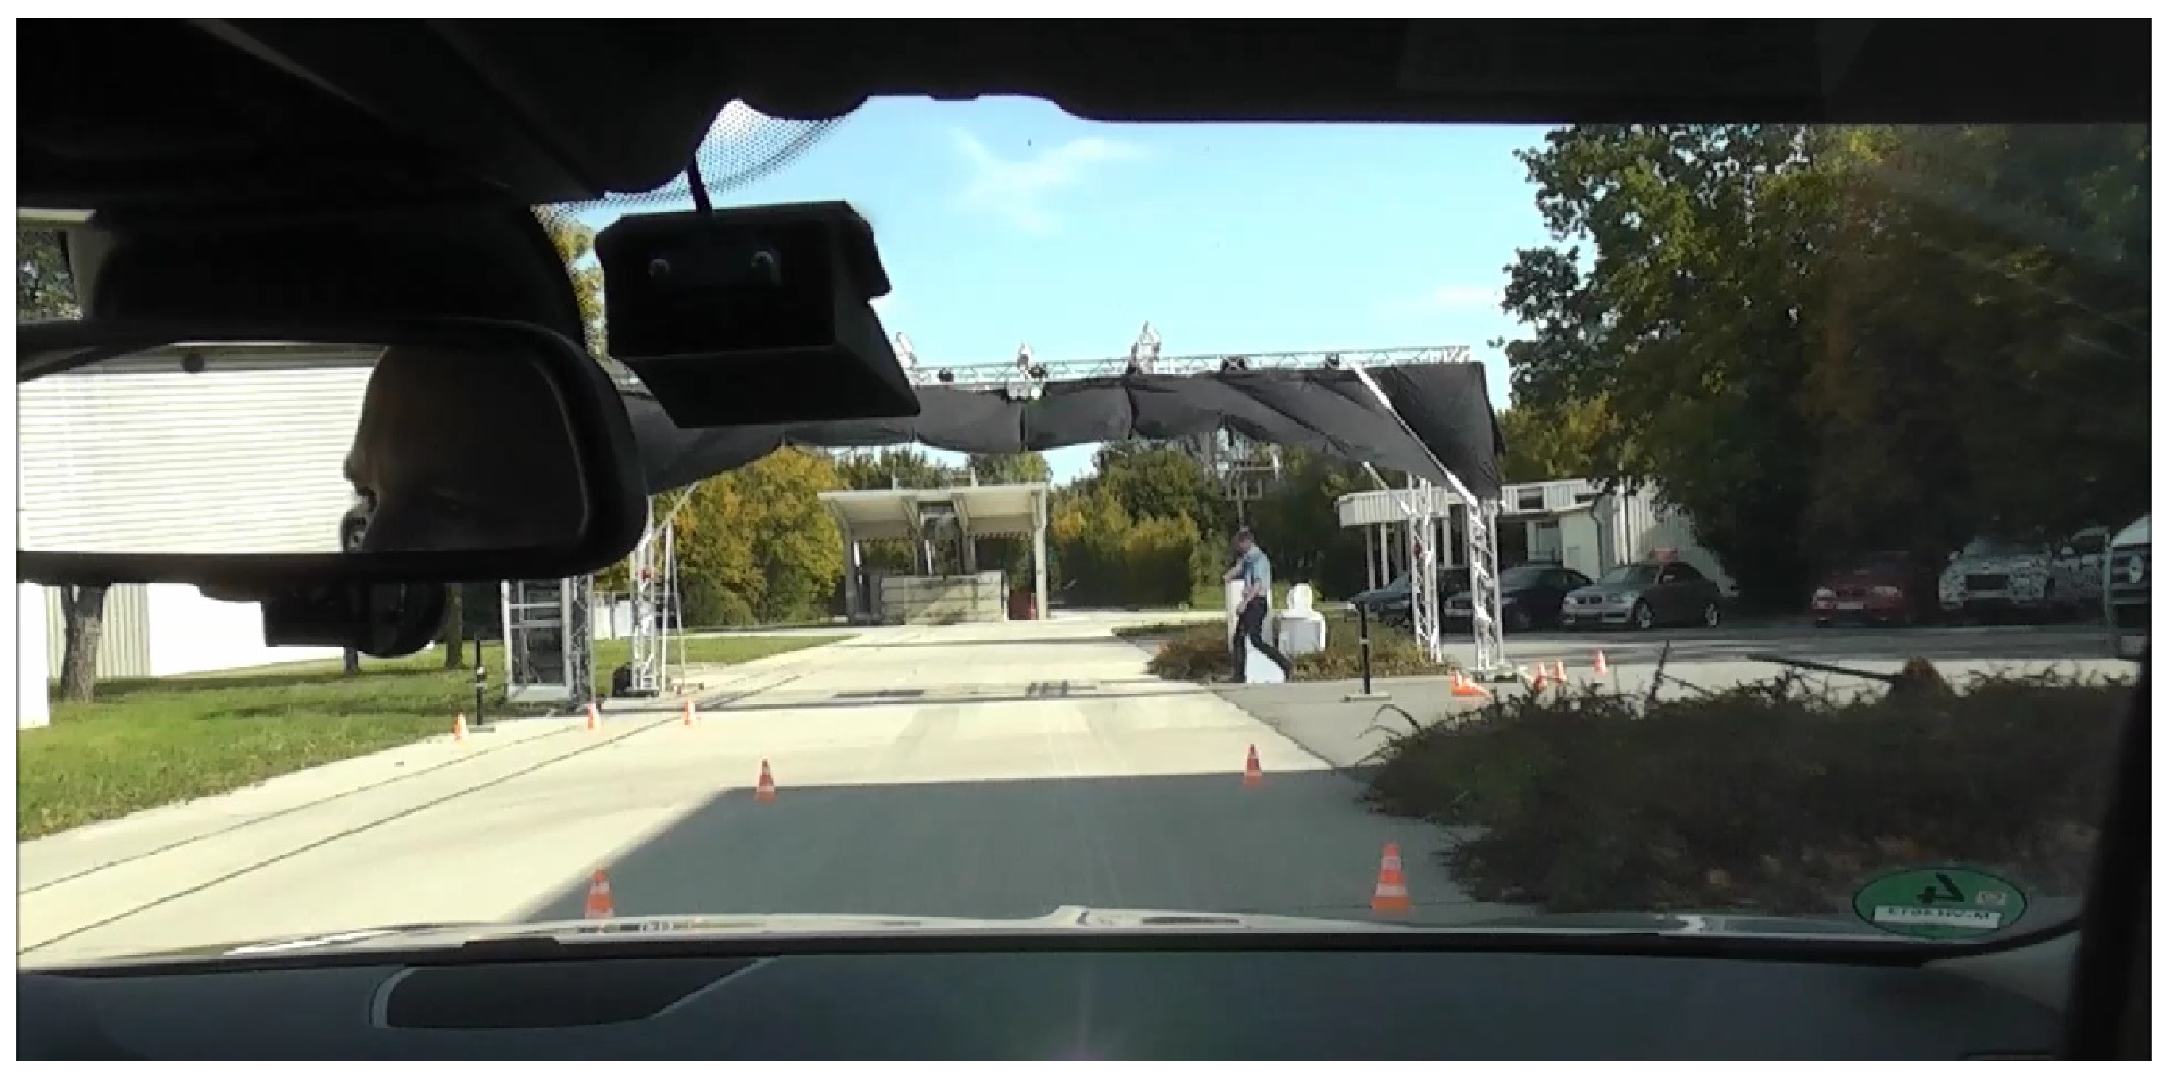
\includegraphics[width=1.\textwidth,clip, trim = 0cm 0cm 0cm 0cm]{6_Innenansicht_Fahrzeug.eps}
\caption[Fahrzeuginnenansicht bei der Anfahrt auf Fußgängerattrappe]{Fahrzeuginnenansicht bei der Anfahrt auf Fußgängerattrappe \citeltex{werling2014riccati}}
\label{fig:Innenansicht_Fahrzeug}
\end{figure}


Zur Visualisierung des Fahrversuchs stellt Abb.\,\ref{fig:draufsicht} vier Momentaufnahmen der Fahrzeugdraufsicht dar. Die detektierte Größe und Position von der stationär\footnote{Die korrekte Funktionsweise des Gesamtsystems wurde ebenfalls mit einem dynamischen Hindernis nachgewiesen. Der dafür erforderliche Prüfstand ist allerdings nicht für die hier demonstrierte Kurvenfahrt geeignet.} installierten Fußgängerattrappe werden durch den dunkelgrauen Kreis repräsentiert. Die beiden hellgrauen Linien zu beiden Seiten des Fahrzeugs stellen den unter Berücksichtigung der Fahrkrümmung und der Außenspiegel prädizierten Fahrkorridor zum Zeitpunkt der Systemaktivierung (schwarzer Punkt) dar. Die optimierte Trajektorie wird zur verbesserten Darstellung durch numerische Simulation des idealen Systemverhaltens als Reaktion auf das optimale Stellgesetz bestimmt und als schwarze Linie gezeichnet. \\
%
Die zu den vier Instantanaufnahmen zugehörigen Signalverläufe der Trajektorienoptimierung werden in Abb.\,\ref{fig:OptimalTrajektorienVerlaeufe} dargestellt. Hierbei wird die optimierte Trajektorie in schwarz, die tatsächliche, zukünftige Trajektorie in grau und die tatsächlich gefahrene Trajektorie gestrichelt gezeichnet. \\
%
Der sich durch das automatische Ausweichmanöver ergebende Winkelverlauf des Lenkrads $\delta_h(t)$ und die Querbeschleunigung $a_q(t)$ sind Abb.\,\ref{fig:LenkwinkelQerbeschleunigungsverlauf} zu entnehmen.%, wobei die in Abb.\,\ref{fig:draufsicht} herausgegriffenen Zeitpunkte durch senkrechte Linien markiert sind. \\


\begin{figure}[!ht]
\centering
% Generated using matlabfrag
% Version: v0.6.16
% Version Date: 04-Apr-2010
% Author: Zebb Prime
%
%% <text>
%
\providecommand\matlabtextA{\color[rgb]{0.000,0.000,0.000}\fontsize{10}{10}\selectfont\strut}%
\psfrag{000}[bc][bc]{\matlabtextA $t=1.76\unit{s}$}%
\psfrag{001}[bc][bc]{\matlabtextA $t=1.07\unit{s}$}%
\psfrag{002}[bc][bc]{\matlabtextA $t=0.42\unit{s}$}%
\psfrag{003}[bc][bc]{\matlabtextA $t=0\unit{s}$}%
%
%% </text>
\renewcommand{\matlabtextA}{\footnotesize}
  	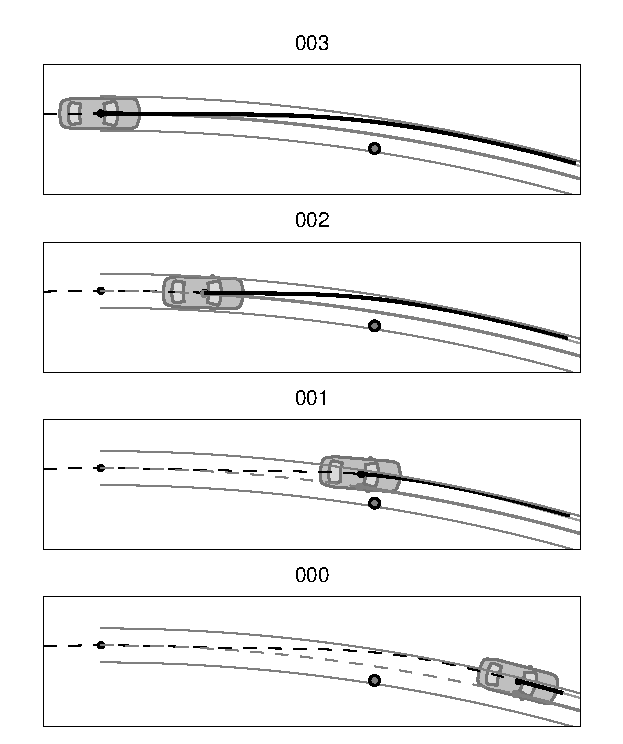
\includegraphics[width=.7\textwidth]{6_Fahrversuch_KurvenAusweichen_topview_riccati.eps}
\def\xlabel{$t$ in \unit{s}}
\caption[Vogelperspektive auf Fahrzeug und Fußgänger]{Vogelperspektive auf Fahrzeug und Fußgänger (dunkelgrauer Punkt) mit optimierter Ausweichtrajektorie (schwarz) und Referenzkorridor (durchgezogen, grau) zu verschiedenen Zeitpunkten \citeltex{werling2014riccati}}
		\label{fig:draufsicht}
\end{figure}
%
\begin{sidewaysfigure}
\centering
% Generated using matlabfrag
% Version: v0.6.16
% Version Date: 04-Apr-2010
% Author: Zebb Prime
%
%% <text>
%
\providecommand\matlabtextA{\color[rgb]{0.000,0.000,0.000}\fontsize{10}{10}\selectfont\strut}%
\psfrag{035}[bc][bc]{\matlabtextA \xlabel}%
\psfrag{036}[bc][bc]{\matlabtextA $t=1.76\unit{s}$}%
\psfrag{037}[bc][bc]{\matlabtextA \xlabel}%
\psfrag{038}[bc][bc]{\matlabtextA $t=1.07\unit{s}$}%
\psfrag{039}[bc][bc]{\matlabtextA \xlabel}%
\psfrag{040}[bc][bc]{\matlabtextA $t=0.42\unit{s}$}%
\psfrag{041}[bc][bc]{\matlabtextA \xlabel}%
\psfrag{042}[tc][tc]{\matlabtextA \ylabelXlat}%
\psfrag{043}[tc][tc]{\matlabtextA \ylabelV}%
\psfrag{044}[tc][tc]{\matlabtextA \ylabelA}%
\psfrag{045}[bc][bc]{\matlabtextA $t=0\unit{s}$}%
\psfrag{046}[tc][tc]{\matlabtextA \ylabelU}%
%
%% </text>
%
%% <xtick>
%
\def\matlabfragNegXTick{\mathord{\makebox[0pt][r]{$-$}}}
%
\psfrag{000}[ct][ct]{\matlabtextA $\matlabfragNegXTick 1$}%
\psfrag{001}[ct][ct]{\matlabtextA $\matlabfragNegXTick 0.5$}%
\psfrag{002}[ct][ct]{\matlabtextA $0$}%
\psfrag{003}[ct][ct]{\matlabtextA $0.5$}%
\psfrag{004}[ct][ct]{\matlabtextA $1$}%
\psfrag{005}[ct][ct]{\matlabtextA $\matlabfragNegXTick 1$}%
\psfrag{006}[ct][ct]{\matlabtextA $\matlabfragNegXTick 0.5$}%
\psfrag{007}[ct][ct]{\matlabtextA $0$}%
\psfrag{008}[ct][ct]{\matlabtextA $0.5$}%
\psfrag{009}[ct][ct]{\matlabtextA $1$}%
\psfrag{010}[ct][ct]{\matlabtextA $\matlabfragNegXTick 1$}%
\psfrag{011}[ct][ct]{\matlabtextA $\matlabfragNegXTick 0.5$}%
\psfrag{012}[ct][ct]{\matlabtextA $0$}%
\psfrag{013}[ct][ct]{\matlabtextA $0.5$}%
\psfrag{014}[ct][ct]{\matlabtextA $1$}%
\psfrag{015}[ct][ct]{\matlabtextA $\matlabfragNegXTick 1$}%
\psfrag{016}[ct][ct]{\matlabtextA $\matlabfragNegXTick 0.5$}%
\psfrag{017}[ct][ct]{\matlabtextA $0$}%
\psfrag{018}[ct][ct]{\matlabtextA $0.5$}%
\psfrag{019}[ct][ct]{\matlabtextA $1$}%
%
%% </xtick>
%
%% <ytick>
%
\psfrag{020}[rc][rc]{\matlabtextA $-1$}%
\psfrag{021}[rc][rc]{\matlabtextA $-0.5$}%
\psfrag{022}[rc][rc]{\matlabtextA $0$}%
\psfrag{023}[rc][rc]{\matlabtextA $0.5$}%
\psfrag{024}[rc][rc]{\matlabtextA $-0.5$}%
\psfrag{025}[rc][rc]{\matlabtextA $0$}%
\psfrag{026}[rc][rc]{\matlabtextA $0.5$}%
\psfrag{027}[rc][rc]{\matlabtextA $1$}%
\psfrag{028}[rc][rc]{\matlabtextA $1.5$}%
\psfrag{029}[rc][rc]{\matlabtextA $-5$}%
\psfrag{030}[rc][rc]{\matlabtextA $0$}%
\psfrag{031}[rc][rc]{\matlabtextA $5$}%
\psfrag{032}[rc][rc]{\matlabtextA $-20$}%
\psfrag{033}[rc][rc]{\matlabtextA $0$}%
\psfrag{034}[rc][rc]{\matlabtextA $20$}%
%
%% </ytick>
\renewcommand{\matlabtextA}{\footnotesize}
	\def\xlabel{$T_\text{tc}$ in \unit{s}}
	\def\ylabelU{$u$ in \unitfrac{m}{$s³$}}		
	\def\ylabelA{$x_3$ in \unitfrac{m}{$s²$}}
	\def\ylabelV{$x_2$ in \unitfrac{m}{s}}	
	\def\ylabelXlat{$x_1$ in  \unit{m}}
  	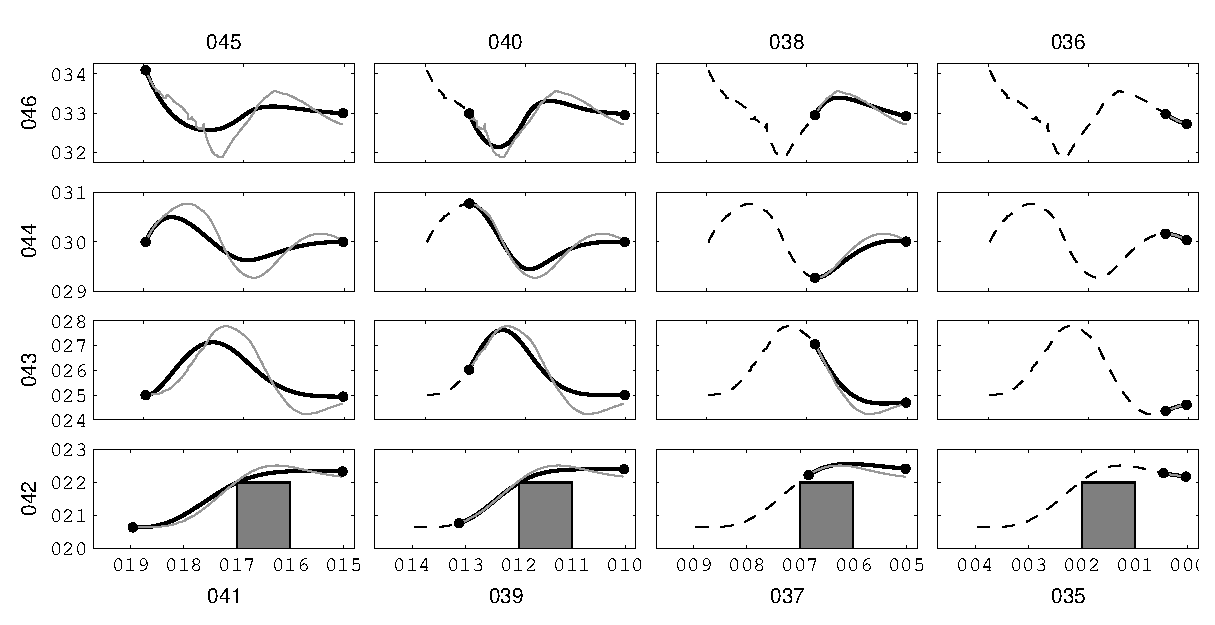
\includegraphics[width=1.\textwidth,clip, trim = 0cm 0cm 0cm 0cm]{6_Fahrversuch_KurvenAusweichen_trajectories.eps}
  \caption[Zustandsverläufe der Trajektorienplanung]{Zustandsverläufe der Trajektorienplanung mit optimierter Trajektorie (schwarz), tatsächliche, zukünftige Trajektorie (grau) und tatsächlich gefahrene Trajektorie (grau gestrichelt) zu den in Abb.\,\ref{fig:draufsicht} dargestellten Zeitpunkten \citeltex{werling2014riccati}}
  \label{fig:OptimalTrajektorienVerlaeufe}
\end{sidewaysfigure}




%
\begin{figure}[!ht]
\centering
% Generated using matlabfrag
% Version: v0.6.16
% Version Date: 04-Apr-2010
% Author: Zebb Prime
%
%% <text>
%
\providecommand\matlabtextA{\color[rgb]{0.000,0.000,0.000}\fontsize{10}{10}\selectfont\strut}%
\psfrag{014}[bc][bc]{\matlabtextA \xlabel}%
\psfrag{015}[tc][tc]{\matlabtextA \ylabelA}%
\psfrag{016}[tc][tc]{\matlabtextA \ylabelB}%
%
%% </text>
%
%% <xtick>
%
\def\matlabfragNegXTick{\mathord{\makebox[0pt][r]{$-$}}}
%
\psfrag{000}[ct][ct]{\matlabtextA $\matlabfragNegXTick 0.5$}%
\psfrag{001}[ct][ct]{\matlabtextA $0$}%
\psfrag{002}[ct][ct]{\matlabtextA $0.5$}%
\psfrag{003}[ct][ct]{\matlabtextA $1$}%
\psfrag{004}[ct][ct]{\matlabtextA $1.5$}%
\psfrag{005}[ct][ct]{\matlabtextA $2$}%
%
%% </xtick>
%
%% <ytick>
%
\psfrag{006}[rc][rc]{\matlabtextA $-6$}%
\psfrag{007}[rc][rc]{\matlabtextA $-4$}%
\psfrag{008}[rc][rc]{\matlabtextA $-2$}%
\psfrag{009}[rc][rc]{\matlabtextA $0$}%
\psfrag{010}[rc][rc]{\matlabtextA $2$}%
\psfrag{011}[rc][rc]{\matlabtextA $-100$}%
\psfrag{012}[rc][rc]{\matlabtextA $-50$}%
\psfrag{013}[rc][rc]{\matlabtextA $0$}%
%
%% </ytick>
%\renewcommand{\matlabtextA}{\footnotesize}
	\def\xlabel{$t$ in \unit{s}}
	\def\ylabelB{$\delta_h$ in \unit{°}}		
	\def\ylabelA{$a_{q}$ in \unitfrac{m}{$s²$}}	
  	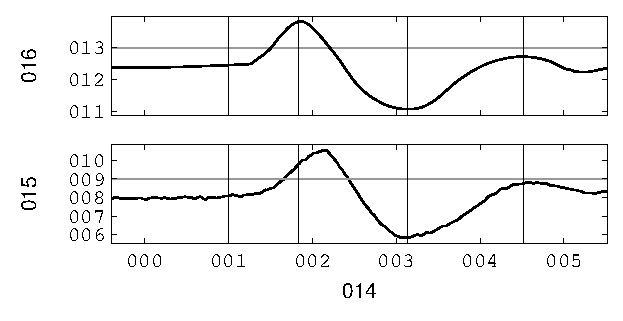
\includegraphics[width=.8\textwidth]{6_Fahrversuch_KurvenAusweichen_signals_delta-a_quer.eps}
  \caption[Zustandsverläufe des ausweichenden Fahrzeugs]{Lenkradwinkel- und Querbeschleunigungsverlauf des ausweichenden Fahrzeugs; die vertikalen Linien markieren die in Abb.\,\ref{fig:draufsicht} dargestellten Zeitpunkte. \citeltex{werling2014riccati}} 
  \label{fig:LenkwinkelQerbeschleunigungsverlauf}
\end{figure}

Zu Versuchsbeginn bewegt sich das manuell gesteuerte Fahrzeug entlang einer Rechtskurve auf den Fußgänger mit etwas über $\unitfrac[40]{km}{h}$ zu. Sobald die $T_\text{tc}$ den parametrierten Schwellwert von einer Sekunde unterschreitet, aktiviert sich das System\footnote{Zur Simulation eines plötzlich die Fahrbahn betretenden Fußgängers wird bis zu dem Zeitpunkt das Kamerasignal unterdrückt, sodass das Fahrzeug nicht frühzeitig die Situation durch Bremsen entschärft.} (s.\ oben in Abb.\,\ref{fig:draufsicht}) und greift in die Lenkung ein, da es für eine kollisionsvermeidende Bremsung zu spät ist. Der kurvenäußere Punkt des Fußgängers ragt zu diesem Zeitpunkt etwa einen halben Meter in den Fahrkorridor, sodass sich zur Vermeidung der Fußgängerkollision mit Sicherheitsabstand eine erforderliche Versatzbreite von $\unit[0.75]{m}$ ergibt. Diese wird durch ein zügiges automatisches Aus- und Gegenlenken (s.\ $\delta_h$-Signal in Abb.\,\ref{fig:LenkwinkelQerbeschleunigungsverlauf}) bis zum Zeitpunkt $T_\text{tc}=0$ auf wenige Zentimeter genau realisiert (s.\ $x_1$-Signal in Abb.\,\ref{fig:OptimalTrajektorienVerlaeufe}). Da eine Stabilisierungsdauer von $t_f- t_1 = \unit[1.0]{s}$ parametriert ist, nutzt das System die Zeit, durch ruhiges Lenken den Fahrzustand entsprechend der manuellen Ursprungskurve zu stabilisieren, s.\ Abb.\,\ref{fig:LenkwinkelQerbeschleunigungsverlauf} bei $t=\unit[2.0]{s}$.


%\subsubsection{Diskussion} \label{sec:diskussion}
Obwohl der unterlagerte Regelkreis die Krümmungssollvorgabe der Trajektorienoptimierung nicht sonderlich genau\footnote{Gründe hierfür sind in der praktischen Anwendung neben Parameterschwankungen vor allem die Fahrerhände am Lenkrad.} umsetzt, s.\ Diskrepanz zwischen geplantem (schwarz) und tatsächlichen Verlauf (grau) vom  $x_3$-Signal in Abb.\,\ref{fig:OptimalTrajektorienVerlaeufe} zum ersten Zeitpunkt, wird dem Fußgänger sicher ausgewichen und das Fahrzeug zuverlässig stabilisiert. Grund hierfür ist die kontinuierliche Optimierung, welche permanent auf die Punktvorgaben für $t_1$ und $t_f$ regelt. Wie dem Zeitpunkt $t=\unit[1.07]{s}$ zu entnehmen ist, wird hierbei kurz vor Erreichen des Zeitpunkts $T_\text{tc}=0$ aufgrund der bereits aufgebauten Versatzgeschwindigkeit das Hindernis ignoriert und direkt auf den Zielzustand umgeschaltet, s.\ Ende Abschn.\,\ref{sec:problemloesung}. Kann darüber hinaus während des Ausweichvorgangs die Fahrzeugsensorik den Fußgänger weiter verfolgen, so muss nicht, wie im vorliegenden Fall,\footnote{Die eingesetzte Sensorik kompensiert die mit einem Ausweichmanöver einhergehende Gier- und Wankbewegung nicht ausreichend genau, sodass in der vorliegenden Implementierung lediglich dem letzten Messwert vor dem Ausweichmanöver vertraut wird.} an der Messinformation zu Manöverbeginn festgehalten werden. Die Neuplanung berücksichtigt dann automatisch in jedem Zeitschritt die aktualisierte Fußgängerprädiktion, sodass die Versatzbreite automatisch angepasst wird und das Fahrzeug auch wirklich nur so viel ausweicht wie zur Kollisionsvermeidung notwendig.
\\
%Ferner wirkt sich aufgrund der kurzen Manöverzeit das Fehlen einer absoluten Positions- und Orientierungsreferenz, wie das GPS, nicht nachteilig aus. %Ferner ist es aufgrund des kurzen Ausweichvorgangs zulässig, auf eine genaue Schwimmwinkelschätzung zu verzichten, da zur Bestimmung der Kurskrümmung $\kappa$ die gemessene Gierrate, Quer- und Längsbeschleunigung die über den integriert werden können.

%Falls der Fußgänger auch während des Ausweichmanövers detektiert werden kann (nicht hier), ist für das Planungsproblem ausschließlich die Ursprungskurve absolute Referenz. Da sind wenige cm nicht wichtig.

%Aus Testfahrersicht scheint unmittelbar vor dem Lenkeingriff eine Kollision mit der Fußgängerattrappe nahezu unausweichlich, sodass es einige Überwindung kostet, nicht manuell einzugreifen. Das Ausweichmanöver selbst fühlt sich jedoch überraschend unspektakulär an, was auch durch die Meinung von Probandenfahrern bestätigt wurde. Im Unterschied zum Ausweichen auf Fahrzeuge, welches i.Allg.\ größere Versatzbreiten und damit höhere Querbeschleunigungen erfordert, verbleibt nämlich typischerweise beim Fußgängerschutzmanöver gar keine Zeit mit dem Fahrzeug hohe Querbeschleunigungen aufzubauen. Vielmehr kommt es auf ein schnelles Lenken an, was von elektrischen Servolenkungen aktuell bereits gut realisiert werden kann. 
%Dies rechtfertigt die in der vorgestellten Trajektorienplanung durchgeführte Vernachlässigung der Querbeschleunigungs- und Stellgrößenbeschränkungen, welche erst die effiziente Berechnung des vorgestellten Ansatzes ermöglicht.
%- Kompromiss aus Versatzbreite und Irritation

%Als weiterführender Schritt ist die Ausweichtrajektorienoptimierung mit unterlagerter Lenkregelung in ein stimmiges Fußgängerschutz-Gesamtkonzept zu integrieren, das entscheidet, ab welchem Zeitpunkt eingegriffen werde kann und ob dann das Ausweichen einem Bremseingriff vorzuziehen ist. Hierbei muss nicht nur die Prädiktion der Fußgängerbewegung, sondern auch die der anderen Verkehrsteilnehmer, insbesondere des Gegenverkehrs, in die Entscheidung einbezogen werden. 

%Durch die hohe Neuplanungsfrequenz: 
%schöne feinfühlig für den Fahrer, der seine Hände am Lenkrad hat, weil permanente neugeplant wird, nicht so wie \cite{werling2012optimal} % Fahrer feinfühlig, Neuplanung zu selten

%Ausweichen ist nur bis zu einer bestimmten Geschwindigkeit sinnvoll; darunter wird gebremst: $v>0$

%Simulation der Hindernistrajektorie damit beliebige Funktionen eingesetzt werden können.

%Vereinfachungen und Einschränkungen: 

%Berücksichtigung von Gegenverkehr, Absicherung etc.
%Physikalische Grenze beim Ausweichen noch nicht erreicht falls nicht vollverzögert wird (s. Ausblick)
%Aufgrund der schnellen Aktordynamik treten in der Praxis keine Stellgrößenbeschränkungen auf

%\subsection{Zusammenfassung}\label{sec:zusammenfassung}
Zusammenfassend kann festgehalten werden, dass zur Vermeidung von Fußgängerkollisionen ein Verfahren vorgestellt wird, das die Ausweichtrajektorienplanung als linear-quadratisches Optimalsteuerungsproblem formuliert und effizient löst. \\
Unter Prädiktion der Fahrzeuglängs- und Fußgängerbewegung wird das Planungsproblem relativ zur ursprünglichen manuellen und i.Allg.\ gekrümmten Fahrkurve formuliert. Dadurch stellt sich die Querbewegung als lineares Integratorsystem dar. Um die Fahrerirritation klein zu halten, darf der Eingriff nur auf einem endlichen Horizont erfolgen, sodass dies von vornherein im Optimierungskriterium berücksichtigt werden muss. Das Optimierungskriterium selbst setzt sich aus zu minimierenden quadratischen Integralkosten bestehend aus Querruck, Quergeschwindigkeit und Querbeschleunigung sowie quadratischen Punktkosten zur Einhaltung des Sicherheitsabstands zum Hindernis und des Fahrzustands am Manöverende zusammen. \\
%Zur Berücksichtigung des Lenkaufwands, des Querbeschleunigungsverlaufs und der Verkehrsgefährdung werden quadratische Integralkosten formuliert. Die Berücksichtigung des Hindernisses sowie des Fahrzeugendzustands erfolgt über sog.\ Punkt- bzw. Endkosten. 
Insgesamt ergibt sich so ein %unrestringiertes 
linear-quadratisches Optimierungsproblem, welches ähnlich zur Riccati-Regelung mit endlichem Optimierungshorizont effizient gelöst werden kann. Durch Parametrierung des Problems über der verbleibenden Zeit bis zum Passieren des Hindernisses kann zusätzlich der rechenintensive Teil der Optimierung vorberechnet werden, sodass sich zur Laufzeit der Rechenaufwand in jedem Zeitschritt auf die Auswertung eines Matrix-Vektor-Produkts reduziert, was bei einer Planungsfrequenz von $\unit[100]{Hz}$ die Echtzeitfähigkeit des Verfahrens bereits auf heutigen Steuergeräten sicherstellt. Die durchgeführten Realversuche mit einer Fußgängerattrappe belegen darüber hinaus die hohe Genauigkeit und Robustheit des optimalen Regelkreises, was auf die permanente Berücksichtigung des Systemzustands in der Optimierung zurückzuführen ist.

%Ein zukünftiger Forschungsschwerpunkt liegt in der Wahl einer geeigneten Bremsstrategie, welche in diesem Beitrag als gegeben angenommen wurde. Da eine Fahrzeugverzögerung dem Fußgänger grundsätzlich mehr Zeit lässt, weiter in den Fahrkorridor einzudringen, liegt hierbei die Herausforderung darin, einen guten Kompromiss zwischen Geschwindigkeitsabbau und erforderlicher Versatzbreite zu finden.

\section{Bewertung}
Auf den ersten Blick erscheint die indirekte Optimierungsmethodik bereits für einfache Problemstellungen sehr aufwändig. Im Unterschied zur direkten Methodik, bei der das Problem "`vorwärts"' implementiert wird und dem Rechner zur Laufzeit die Optimierung der Zustands- und Stellgrößenverläufe überlassen wird, ist bei der indirekten Methode das Optimierungsproblem vorab in ein Randwertproblem überzuführen, was je nach Aufgabenstellung mehr oder weniger "`Handarbeit"' erfordert. Für elementare Standardmanöver, bei denen das Fahrzeug als Punktmasse modelliert wird, können jedoch geschlossene Lösungen gefunden werden, deren Berechnung zur Programmlaufzeit einen minimalen Aufwand bedeutet. Das ermöglicht die effiziente Einbettung der Elementarmanöver in übergeordnete Optimierungsroutinen mit vielfältigen Einsatzmöglichkeiten. So werden in \citeltex{werling2012optimal} die in Abschn.\,\ref{sec:polytraj} hergeleiteten Optimaltrajektorien zur Berechnung quer-längs-gekoppelter Manöver zwischen beweglichen Hindernissen herangezogen, indem durch geeignetes Sampling über eine Vielzahl möglicher Zielzustände und Endzeitpunkte optimiert wird. In leicht abgeänderter Form findet der Algorithmus auch Anwendung bei der Prädiktion von Fremdfahrzeugen \cite{houenou2013vehicle} und der Simulation ganzer Verkehrsflüsse \cite{xu2011micro}. \\
Des Weiteren stellen schnell berechenbare Elementarlösungen geeignete Distanzmaße dar \cite{soueres1998optimal}, um bei der gerichteten Suche in Abschn.\,\ref{sec:astern} als Heuristik das Auffinden der Optimallösung enorm zu beschleunigen, s.\ hierzu Kap.\,\ref{chap:dynamische_Optimierung_dynamisch}. %\\

%Anmerkung: Nebenbedingungen sind bei der indirketen Methode schwer zu berücksichtigen: Heuristik für A* kann durch relaxation des Ursprungsproblems gefunden werden. Wenn diese Relaxiation dazu führt, dass geschlossene Lösungen gefunden werden, dann ist indirekte Methode eine klasse Kombination.


Die Aufgabenstellung kann darüber hinaus durch zusätzliche Nebenbedingungen für interne Randpunkte, Zustände oder Eingänge an weitere praktische Anforderungen angepasst werden, wenn auch mit ungleich größerem Aufwand als bei den direkten Methoden. Das hat aber zur Folge, dass in den allermeisten Fällen, wie auch in Abschn.\,\ref{sec:zustandsbeschraenkung_hamilton}, die hinzukommenden algebraischen Gleichungen numerisch gelöst werden müssen, was den Online-Rechenaufwand erhöht, insbesondere wenn Lösungen (der nur notwendigen Gleichungen) auftreten, die nicht Lösung des Optimalsteuerungsproblems sind.

%Schließlich ist es möglich, die Herangehensweise der Riccati-Regelung mit endlichem Horizont auf das Manöverplanungsproblem zu übertragen. Hierdurch können lineare Fahrzeugmodelle (z.B. linearisiertes Einspurmodell) mit quadratischen Kostenfunktionalen kombiniert werden und das Optimalsteuerungsproblem effizient und numerisch-robust gelöst werden.

% Analytische Expansionen: stangl armin

Beim Entwurf neuer Fahrfunktionen steht der Entwickler folglich vor der Aufgabe zu entscheiden, ob aus der übergeordneten Problemstellung elementare Teilaufgaben isoliert werden können, die sich so übersichtlich darstellen, dass die indirekte Methodik gewinnbringend eingesetzt werden kann. Falls dann der Weg über die indirekte Methodik eingeschlagen wird, sich aber neue Anforderungen ergeben, so verbleibt immer noch die Möglichkeit, die Aufgabenstellung mit geeignet gewählten internen Randpunkten und weiteren Nebenbedingungen anzupassen.

Insbesondere bei nichtlinearen Problemen ist es schwierig, die Hamilton-Differentialgleichung geschlossen zu lösen, sodass der Ingenieur dann darauf angewiesen ist, das Randwertproblem numerisch zu lösen (vgl.\ Abschn.\,\ref{sec:loesung_direkt_numerisch}).  Als indirekte Optimierungsmethoden existieren hierzu Diskretisierungs-, Schieß- oder Gradientenverfahren (s.\ \cite{papageorgiou2012optimierung} und für die praktische Umsetzung z.B.\ \cite{graichen_suboptimal}). Da die Verfahren noch nicht den Bekanntheitsgrad der direkten Methode genießen, verwundert es nicht, dass zurzeit keine Anwendungen im Fahrzeugumfeld bekannt sind, sodass auf deren Darstellung verzichtet wird. Angesichts der Tatsache, dass die genannten Verfahren i.Allg.\ keine Zusatzsoftware (wie etwa Sequentielle Quadratische Programme bei der direkten Methode) erfordern, die eine Zertifizierung des Fahrerassistenzsystems erschwert, besteht hier Forschungsbedarf.


%Von der Trajektorienplanung im Fahrzeugumfeld aktuell völlig ungeachtet sind numerische Methoden


\cleardoublepage
